\documentclass[10pt,journal,compsoc]{IEEEtran}

\usepackage{cite}
\usepackage{amsmath,amssymb,amsfonts,amsthm,amscd,bm,bbm}
\usepackage{mathtools}
%\mathtoolsset{showonlyrefs}
%\usepackage[inline]{enumitem}
\usepackage[pdftex]{graphicx}
\graphicspath{{./figs/}}
\usepackage{algorithmic}
\usepackage{algorithm}
%\usepackage[none]{hyphenat}
\usepackage{multirow}
\usepackage{colortbl}
\usepackage{array,booktabs}
\usepackage{xcolor}
\usepackage{makecell}
\usepackage{pifont}
\newcommand{\cmark}{\ding{51}}
\newcommand{\xmark}{\ding{55}}

\newtheorem{theorem}{Theorem}
\newtheorem{definition}[theorem]{Definition}
\newtheorem{assumption}[theorem]{Assumption}
\newtheorem{lemma}[theorem]{Lemma}
\newtheorem{corollary}[theorem]{Corollary}
\newtheorem{proposition}[theorem]{Proposition}
\newtheorem{conjecture}[theorem]{Conjecture}
\newtheorem{remark}[theorem]{Remark}
\newtheorem{example}{Example}

\DeclareMathOperator{\aff}{aff}
\DeclareMathOperator{\st}{s.t.}
\DeclareMathOperator{\affnot}{aff_0}
\DeclareMathOperator{\conv}{conv}
\DeclareMathOperator{\relint}{relint}
\DeclareMathOperator{\vol}{vol}
\DeclareMathOperator{\range}{range}
\DeclareMathOperator{\image}{im}
\DeclareMathOperator{\nullspace}{null}
\DeclareMathOperator{\area}{area}
\DeclareMathOperator{\vspan}{span}
\DeclareMathOperator{\id}{Id}
\DeclareMathOperator{\cond}{cond}
\DeclareMathOperator{\prox}{prox}
\DeclareMathOperator*{\argmax}{arg\,max}
\DeclareMathOperator*{\argmin}{arg\,min}
\DeclareMathOperator*{\minimize}{minimize}
\DeclareMathOperator{\diag}{diag}
\DeclareMathOperator{\Tr}{Tr}

\newcommand\Energy{\mathcal{E}}
\newcommand\EnergyH{\mathcal{E}^{H}}
\newcommand\EnergyL{\mathcal{E}^{L}}
\newcommand\EnergyOne{\mathcal{E}^{1D}}
\newcommand\E{\mathbb{E}}
\newcommand\kk{K}
\newcommand\kkk{h}
\newcommand\Hk{{\mathcal{H}}_{\kk}}
\newcommand\HH{\mathcal{H}}
\newcommand\C{{\mathcal{C}}}
\newcommand\tC{{\widetilde{\C}}}
\newcommand\OO{{\mathcal{O}}}
\newcommand\W{{\mathcal{W}}}
\newcommand\Zt{Y}
\newcommand{\Ind}[1]{\mathbbm{1}_{#1}}
\newcommand\e{e}
\newcommand\om{\omega}


\hyphenation{op-tical net-works semi-conduc-tor}

\begin{document}

\title{Kernel k-Groups via Hartigan's Method}

\author{Guilherme~Fran\c ca,~Maria Rizzo~and~Joshua T.~Vogelstein
\IEEEcompsocitemizethanks{\IEEEcompsocthanksitem G. Fran\c ca 
and J. Vogelstein are with the Center for Imaging Science, Johns Hopkins
University; J. Vogelstein is also with 
the Department of Biomedical Engineering and Institute for Computational
Medicine, Johns Hopkins University. \protect\\
% note need leading \protect in front of \\ to get a newline within \thanks as
% \\ is fragile and will error, could use \hfil\break instead.
E-mail: guifranca@jhu.edu; jovo@jhu.edu
\IEEEcompsocthanksitem M. Rizzo is with the Department of Mathematics
and Statistics, Bowling Green State University. \protect\\
E-mail: mrizzo@bgsu.edu}% <-this % stops an unwanted space
\thanks{Manuscript received March 15, 2018; revised March 15, 2018.}}

% The paper headers
\markboth{Energy Clustering}{}
%{Journal of \LaTeX\ Class Files,~Vol.~14, No.~8, August~2015}%


\IEEEtitleabstractindextext{%
\begin{abstract}
Energy statistics was proposed by Sz\' ekely in the 80's inspired by 
Newton's gravitational potential in classical mechanics, and it provides
a model-free 
hypothesis test for equality of distributions. In its original form, energy
statistics was formulated in 
Euclidean spaces. More recently, it 
was generalized to metric spaces of negative type. 
In this paper, we consider a formulation for the clustering problem
using a weighted version of 
energy statistics in spaces of negative type.
We show that this approach leads to a
quadratically constrained
quadratic program in the associated kernel space, establishing
connections with graph partitioning problems and
kernel methods in unsupervised machine learning.
To find local solutions of such an optimization problem, 
we propose an extension of Hartigan's method to kernel spaces.
Our method has the same computational cost
as kernel k-means algorithm, which is based on Lloyd's heuristic, but 
our numerical results show an improved performance,
especially in high dimensions.
\end{abstract}

% Note that keywords are not normally used for peerreview papers.
\begin{IEEEkeywords}
Clustering, Energy Statistics, Kernel Methods.
\end{IEEEkeywords}}


% make the title area
\maketitle


% To allow for easy dual compilation without having to reenter the
% abstract/keywords data, the \IEEEtitleabstractindextext text will
% not be used in maketitle, but will appear (i.e., to be "transported")
% here as \IEEEdisplaynontitleabstractindextext when the compsoc 
% or transmag modes are not selected <OR> if conference mode is selected 
% - because all conference papers position the abstract like regular
% papers do.
\IEEEdisplaynontitleabstractindextext
% \IEEEdisplaynontitleabstractindextext has no effect when using
% compsoc or transmag under a non-conference mode.



% For peer review papers, you can put extra information on the cover
% page as needed:
% \ifCLASSOPTIONpeerreview
% \begin{center} \bfseries EDICS Category: 3-BBND \end{center}
% \fi
%
% For peerreview papers, this IEEEtran command inserts a page break and
% creates the second title. It will be ignored for other modes.
\IEEEpeerreviewmaketitle



\IEEEraisesectionheading{\section{Introduction}\label{sec:introduction}}
% Computer Society journal (but not conference!) papers do something unusual
% with the very first section heading (almost always called "Introduction").
% They place it ABOVE the main text! IEEEtran.cls does not automatically do
% this for you, but you can achieve this effect with the provided
% \IEEEraisesectionheading{} command. Note the need to keep any \label that
% is to refer to the section immediately after \section in the above as
% \IEEEraisesectionheading puts \section within a raised box.




% The very first letter is a 2 line initial drop letter followed
% by the rest of the first word in caps (small caps for compsoc).
% 
% form to use if the first word consists of a single letter:
% \IEEEPARstart{A}{demo} file is ....
% 
% form to use if you need the single drop letter followed by
% normal text (unknown if ever used by the IEEE):
% \IEEEPARstart{A}{}demo file is ....
% 
% Some journals put the first two words in caps:
% \IEEEPARstart{T}{his demo} file is ....
% 
% Here we have the typical use of a "T" for an initial drop letter
% and "HIS" in caps to complete the first word.


\IEEEPARstart{E}{nergy Statistics} \cite{Szkely2013,Szkely2017}
is based on a 
notion of statistical potential energy between probability distributions,
in close analogy to Newton's gravitational potential in classical mechanics.
When probability distributions are different, the 
``statistical potential energy'' diverges as sample size increases, 
while tends 
to a nondegenerate limit distribution when probability
distributions are equal. 
Thus, it provides a model-free hypothesis test for equality of 
distributions which is achieved under minimum energy. 

Energy statistics has been applied to several goodness-of-fit 
hypothesis tests, multi-sample tests of equality of distributions, 
analysis of variance \cite{RizzoVariance}, nonlinear dependence tests through
distance covariance and distance correlation~\cite{Szekely2007-mm}, which generalizes the Pearson
correlation coefficient, and hierarchical clustering 
by extending Ward's method of minimum variance
\cite{RizzoClustering}; 
see \cite{Szkely2013,Szkely2017} for an overview of energy
statistics and its applications.
Moreover, in Euclidean spaces, an application of 
energy statistics to clustering
was recently proposed \cite{Kgroups}, and the method was named 
\emph{k-groups}. 

In its original formulation, energy statistics has a compact representation
in terms of expectations of pairwise Euclidean distances, providing
straightforward empirical estimates. 
More recently, the notion of distance covariance was further 
generalized from Euclidean 
spaces to metric spaces of negative type \cite{Lyons}. Furthermore, 
the link between energy distance based tests and kernel 
based tests has 
been recently established \cite{Sejdinovic2013} 
through an asymptotic equivalence between generalized energy distances and maximum
mean discrepancies (MMD), which are distances between embeddings of 
distributions in reproducing kernel Hilbert spaces (RKHS).
Even more recently, generalized energy distances and kernel methods have been demonstrated to be exactly equivalent, for all finite samples~\cite{Shen2018-st}.
This equivalence immediately relates energy statistics to
kernel methods often used in machine learning, and form the basis 
of our approach in this paper.

Clustering is an important unsupervised learning problem and 
has a long history in statistics and machine learning, making it
impossible to mention all important contributions in a short space. 
Perhaps, the most used method is k-means \cite{Lloyd,MacQueen,Forgy}, which
is based on Lloyd's heuristic \cite{Lloyd} of iteratively computing
the means of each cluster and then assigning points to
the cluster with closest center. The only statistical 
information about each cluster comes from its mean, making the method sensitive 
to outliers. Nevertheless, k-means works very well when data is 
linearly separable in Euclidean space. Gaussian mixture models (GMM) is 
another very common approach, providing more flexibility than k-means; 
however, it still makes strong assumptions about the distribution of 
the data.

To account for nonlinearities, kernel methods were introduced 
\cite{Smola,Girolami}. A Mercer kernel \cite{Mercer} is used to implicitly
map data points to a RKHS, then clustering can be performed in the associated
Hilbert space by using its inner product. However, the kernel choice remains 
the biggest challenge since there is no principled theory to construct a kernel
for a given dataset, and usually a kernel introduces hyperparameters that 
need to be carefully chosen. A well-known kernel based clustering method
is kernel k-means, which is precisely k-means 
formulated in the feature space \cite{Girolami}. 
Furthermore, kernel k-means algorithm
\cite{Dhillon2,Dhillon} is still based on Loyd's heuristic.
We refer the reader to \cite{Filippone} for a survey of clustering
methods.

Besides Lloyd's approach to clustering %, in Euclidean or kernel spaces,
there is an old heuristic
due to Hartigan \cite{Hartigan1975,Hartigan1979} that
goes as follows: for each data point, simply assign it to a cluster
in an optimal way such that a loss function is minimized.
While Lloyd's method only iterates if some cluster contains a point
that is closer to the mean of another cluster, Hartigan's method may iterate
even if that is not the case, and moreover, it takes into account the motion
of the means resulting from the reassignments. In this sense, Hartigan's
method may potentially escape local minima of Lloyd's method.
In the Euclidean case, this was shown to be the case \cite{Telgarsky}.
Moreover, the advantages of Hartigan's over Lloyd's method was verified
empirically \cite{Telgarsky,Slonin}. However, 
although it was observed to be as fast as Lloyd's method, no complexity
analysis was provided. 


\subsection*{Contributions}
Although k-groups considers clustering from energy statistics
in the particular Euclidean case \cite{Kgroups},
the precise optimization problem behind this approach
remains obscure, as well as the connection with other methods
in machine learning.
The main theoretical contribution of this paper is to fill these gaps, 
which 
we do   more generality. For instance, our approach is not limited
to the Euclidean case but holds for general arbitrary spaces
of negative type. 
For generality, we also
consider a weighted version of energy statistics.
Our approach reveals connections
between energy statistics based clustering and existing methods
such as kernel k-means and graph partitioning problems.

Another contribution of this paper is to extend 
Hartigan's method to  kernel spaces. 
To the best of our knowledge, such an extension was not previously considered.
Since this approach was motivated by energy statistics and  
\cite{Kgroups} considered the Euclidean case, we call the 
proposed method \emph{kernel k-groups}.
We show that kernel k-groups 
has the same complexity as kernel k-means algorithm, however,
our numerical results provide compelling evidence that 
kernel k-groups 
is more accurate and robust, especially in high dimensions. 

Using the standard kernel defined by energy
statistics, our experiments illustrate 
that kernel k-groups
is able to perform accurately on data coming from 
very different distributions, contrary to k-means and GMM, for instance.
More specifically, our method performs 
closely to k-means and GMM on normally distributed data, while
it is significantly better on data that 
is not normally distributed. 
Its superiority in high dimensions
is striking, being more accurate than k-means and GMM 
even in Gaussian settings. We also illustrate the advantages of
kernel k-groups on real data. 


%%%%%%%%%%%%%%%%%%%%%%%%%%%%%%%%%%%%%%%%%%%%%%%%%%%%%%%%%%%%%%%%%%%%%%%%%%%%%%%
\section{Review of Energy Statistics and RKHS}
\label{sec:background}

In this section, we introduce the main concepts from energy
statistics and its relation to 
RKHS which form the basis of our work.
For more details we refer 
to \cite{Szkely2013} and \cite{Lyons,Sejdinovic2013}.

Consider random variables in $\mathbb{R}^D$ 
such that $X,X' \stackrel{iid}{\sim} P$ and 
$Y,Y' \stackrel{iid}{\sim} Q$, where $P$ and $Q$ are cumulative
distribution functions with finite first moments. 
The quantity 
\begin{equation}
\label{eq:energy}
\Energy(P, Q) \equiv 2 \E \| X - Y\| - \E \| X - X' \| - \E \| Y - Y' \|,
\end{equation}
called \emph{energy distance} \cite{Szkely2013}, 
is rotationally invariant and nonnegative, $\Energy(P,Q) \ge 0$, where
equality
to zero holds if and only if $P = Q$.
Above, $\| \cdot \|$ denotes the
Euclidean norm in $\mathbb{R}^D$. 
Energy distance
provides a characterization of equality of distributions, and
$\Energy^{1/2}$ is
a metric on the space of distributions.

The energy distance can be generalized as, for instance,
\begin{equation}
\label{eq:energy2}
\Energy_\alpha(P, Q) \equiv 
2 \E \| X - Y\|^{\alpha} - \E \| X - X' \|^{\alpha} - 
\E \| Y - Y' \|^{\alpha}
\end{equation}
where $0<\alpha\le 2$. This quantity is also nonnegative,
$\Energy_\alpha(P,Q) \ge 0$. Furthermore, for $0<\alpha<2$ we have that
$\Energy_\alpha(P,Q) = 0$ if and only if $P=Q$, while for $\alpha=2$ 
we have $\Energy_2(P,Q) = 2\| \E(X) - \E(Y) \|^2$ which shows that
equality to zero only requires
equality of the means, and thus $\Energy_2(P,Q)=0$ does 
not imply equality of distributions. 

The energy distance can be even further generalized.
Let $X, Y \in \mathcal{X}$  where $\mathcal{X}$ is an arbitrary space endowed
with a \emph{semimetric of negative type}
$\rho: \mathcal{X}\times\mathcal{X} \to \mathbb{R}$, which is required
to satisfy
\begin{equation}
\label{eq:negative_type}
\sum_{i,j=1}^n c_i c_j \rho(X_i, X_j) \le 0,
\end{equation}
where $X_i \in \mathcal{X}$ and $c_i \in \mathbb{R}$ such that
$\sum_{i=1}^n c_i = 0$. Then, $\mathcal{X}$ is called a \emph{space of
negative type}.
We can thus replace $\mathbb{R}^D$ by $\mathcal{X}$ and 
$\| X - Y \|$ by $\rho(X , Y)$ in the definition \eqref{eq:energy}, obtaining
the \emph{generalized energy distance}
\begin{equation}
\label{eq:energy3}
\Energy(P, Q) \equiv 2 \E \rho(X,Y) - \E \rho(X, X') - \E \rho(Y,Y').
\end{equation}
For spaces of negative type, there exists a Hilbert space $\mathcal{H}$ and
a map $\varphi: \mathcal{X} \to
\mathcal{H}$ such that
$\rho(X, Y) = \| \varphi(X) - \varphi(Y) \|_{\mathcal{H}}^2$. This
allows us to compute quantities related to probability distributions over
$\mathcal{X}$ in the associated Hilbert space $\mathcal{H}$.
Even though the semimetric 
$\rho$ may not satisfy the triangle inequality, 
$\rho^{1/2}$ does since it can be shown to be a proper metric. 
Our energy clustering formulation, proposed in the next section,
will be based on the generalized
energy distance \eqref{eq:energy3}.

There is an equivalence between energy distance, 
commonly used in statistics,
and distances between embeddings of distributions in 
RKHS, commonly used in machine learning. 
This equivalence was established
in \cite{Sejdinovic2013}. Let us first recall the definition of
RKHS. Let $\HH$ be a Hilbert space of real-valued functions
over $\mathcal{X}$. A function 
$\kk : \mathcal{X} \times \mathcal{X} \to 
\mathbb{R}$ is a reproducing kernel of $\HH$ if it satisfies
the following two conditions:
\begin{enumerate}
\item $\kkk_x \equiv \kk(\cdot, x) \in \HH$ 
for all $x \in \mathcal{X}$;
\item $\langle \kkk_x, f \rangle_{\HH} = f(x)$ for
all $x\in\mathcal{X}$ and $f\in \HH$.
\end{enumerate}
In other words, for any $x \in \mathcal{X}$ and any function $f \in \HH$,
there is a unique 
$\kkk_x \in \HH$ that reproduces $f(x)$ through the inner product
of $\HH$.
If such a \emph{kernel} 
function $\kk$ exists, then $\HH$ is called a RKHS. The above two 
properties immediately imply that $\kk$ is symmetric and positive
definite. 
Defining the Gram matrix $G$ with
elements $G_{ij} = \kk(x_i,x_j)$, this is equivalent to $G=G^\top$ being
positive semidefinite, i.e., $v^\top G \, v \ge 0$ for any vector
$v \in \mathbb{R}^n$.

The Moore-Aronszajn theorem 
\cite{Aronszajn}
establishes the converse of the above paragraph.
For every symmetric
and positive definite function $\kk: \mathcal{X}\times \mathcal{X} \to
\mathbb{R}$, there is an associated RKHS, $\Hk$,
with reproducing
kernel $\kk$. The map $\varphi: x \mapsto \kkk_x \in \Hk$ is called
the canonical \emph{feature map}. Given a kernel $\kk$,
this theorem enables us to define an embedding of a probability measure
$P$ into the RKHS as follows: $P \mapsto \kkk_P \in
\Hk$ such that 
$\int f(x) d P(x) = \langle f, \kkk_P \rangle$ for all $f \in \Hk$,
or alternatively, $\kkk_P \equiv \int \kk( \, \cdot \,, x)  d P(x)$. 
We can now  introduce the 
notion of distance between two probability measures using the inner product
of $\Hk$, which is called the maximum mean discrepancy (MMD) and
is given by
\begin{equation}
\label{eq:mmd}
\gamma_\kk(P,Q) \equiv \| \kkk_P - \kkk_Q \|_{\Hk}.
\end{equation}
This can also be written as \cite{Gretton2012}
\begin{equation}\label{eq:mmd2}
\gamma_\kk^2(P,Q) = \E \kk(X,X') + \E \kk(Y,Y') - 2 \E \kk(X, Y)
\end{equation}
where $X,X' \stackrel{iid}{\sim} P$ and $Y,Y'\stackrel{iid}{\sim} Q$.
From the equality between \eqref{eq:mmd} and \eqref{eq:mmd2} we also
have $\langle \kkk_P, \kkk_Q \rangle_{\Hk} = \E \, \kk(X, Y)$.

The following important result shows that semimetrics of negative
type and symmetric positive definite kernels are closely related
\cite{Berg1984}. Let $\rho: \mathcal{X} \times \mathcal{X} \to \mathbb{R}$
and $x_0 \in \mathcal{X}$ an arbitrary but fixed point.
Define
\begin{equation}
\label{eq:kernel_semimetric}
\kk(x,y) \equiv 
\tfrac{1}{2} \left[  \rho(x,x_0) + \rho(y,x_0) - \rho(x,y)\right].
\end{equation}
Then, it can be shown that 
$\kk$ is positive definite if and only if $\rho$ is a semimetric
of negative type.
We have a family of kernels, one for each choice of $x_0$. Conversely,
if $\rho$ is a semimetric of negative type and $\kk$ is a kernel in this
family, then 
\begin{equation}
\label{eq:gen_kernel}
\begin{split}
\rho(x,y) &= \kk(x,x) + \kk(y,y) -2\kk(x,y) \\
&=  \| \kkk_x - \kkk_y \|^2_{\Hk}
\end{split}
\end{equation}
and the canonical feature map 
$\varphi: x \mapsto \kkk_x$ is injective \cite{Sejdinovic2013}.
When these conditions are satisfied, we say that the kernel $\kk$ 
generates the semimetric $\rho$. 
If two different kernels generate the same $\rho$, they are
said to be equivalent kernels.

Now we can state the equivalence between the generalized 
energy distance \eqref{eq:energy3} and
inner products on RKHS, which is one of the main results of
\cite{Sejdinovic2013}. If $\rho$ is a semimetric
of negative type and $\kk$ a kernel that generates $\rho$, then
replacing \eqref{eq:gen_kernel} into
\eqref{eq:energy3}, and using \eqref{eq:mmd2}, yields
\begin{equation} \label{eq:Erho}
\begin{split}
\Energy(P, Q) &= 
2 \left[ \E \, \kk(X, X') + \E \, \kk(Y, Y') - 2\E \, \kk(X, Y)\right]  \\
&= 2 \gamma_\kk^2(P,Q) .
\end{split}
\end{equation}
Due to \eqref{eq:mmd}, we can compute the energy 
distance $\mathcal{E}(P, Q)$ between two probability distributions
using the inner 
product of $\Hk$. 

Finally, let us recall the main formulas from generalized energy statistics
for the test statistic of equality of distributions \cite{Szkely2013}. 
Assume that we have data $\mathbb{X} = \{ x_1,\dotsc, x_n \}$, where
$x_i \in \mathcal{X}$, and $\mathcal{X}$ is a space of negative type.
Consider a disjoint partition $\mathbb{X} = \bigcup_{j=1}^k \C_j$, with
$\C_i \cap \C_j = \emptyset$.
Each expectation in the generalized energy distance
\eqref{eq:energy3}
can be computed 
through the function
\begin{equation}
\label{eq:g_def}
g (\C_i, \C_j) \equiv 
\dfrac{1}{n_i n_j}
\sum_{x \in \C_i} 
\sum_{y \in \C_j} \rho(x, y) ,
\end{equation}
where $n_i = |\C_i|$ is the number of elements in partition
$\C_i$. 
The \emph{within energy dispersion} is defined by
\begin{equation}
\label{eq:within}
W \equiv
\sum_{j=1}^{k} \dfrac{n_j}{2} g(\C_j, \C_j),
\end{equation}
and the \emph{between-sample energy statistic} is defined by
\begin{equation}
\label{eq:between}
S \equiv \!\!\!\!
\sum_{1 \le  i < j \le k } \dfrac{n_i n_{j}}{2 n} \left[
2 g(\C_i, \C_j) - 
g(\C_i, \C_i) - 
g(\C_j, \C_j)
\right],
\end{equation}
where $n = \sum_{j=1}^k n_j$.
Given a set of distributions
$\{ P_j\}_{j=1}^k$, where $x \in \C_j$ if and only if $x \sim P_j$, 
the quantity $S$ provides
a test statistic for equality of distributions
\cite{Szkely2013}.
When the sample size is large enough, $n\to \infty$,
under the null hypothesis $H_0: P_1=P_2=\dotsm=P_k$, we have that
$S\to 0$, 
and under
the alternative hypothesis $H_1: P_i \ne P_j$ for at least two $i\ne j$, 
we have that $S \to \infty$.
%Note that this test does not make any assumptions
%about the form of distribution $P_j$, thus it is said to be 
%distribution-free.

%One can make a physical analogy by thinking 
%that points $ x \in \C_j$ form a massive body 
%whose total mass is characterized by the distribution function $P_j$.
%The quantity $S$ is thus a potential
%energy of the from $S(P_1,\dotsc,P_k)$ which measures how different
%the distribution of these masses are,  and achieves the ground state
%$S=0$ when all bodies have the same mass distribution. On the other hand,
%the potential energy
%$S$ increases as bodies have different mass distributions.


%%%%%%%%%%%%%%%%%%%%%%%%%%%%%%%%%%%%%%%%%%%%%%%%%%%%%%%%%%%%%%%%%%%%%%%%%%%%%%%
\section{The Clustering Problem Formulation}
\label{sec:clustering_theory}

This section contains our main theoretical results. First, we
generalize the previous formulas from energy statistics by introducing
weights associated to data points. 
Second, we formulate an optimization problem for clustering 
in the associated RKHS, making connection with kernel methods in
machine learning. 

Let $w(x)$ be a weight function associated to point $x \in \mathcal{X}$
and define
\begin{equation}
\label{eq:g_def2}
g(\C_i, \C_j) \equiv \dfrac{1}{s_i s_j} \sum_{x\in \C_i}\sum_{y\in\C_j}
w(x)w(y) \rho(x,y),
\end{equation}
where
\begin{equation}
s_i \equiv \sum_{x\in\C_i} w(x), \qquad
s \equiv \sum_{j=1}^k s_j.
\end{equation}
The  weighted version of the within energy dispersion 
and between-sample
energy statistic are thus given by
\begin{align}
W &\equiv
\sum_{j=1}^{k} \dfrac{s_j}{2} g(\C_j, \C_j), \label{eq:within2} \\
S &\equiv \!\!\! \sum_{1 \le  i < j \le k } \!\!\! 
\dfrac{s_i s_{j}}{2 s} \left[
2 g(\C_i, \C_j) - 
g(\C_i, \C_i) - 
g(\C_j, \C_j)
\right]. \label{eq:between2}
\end{align}
Note that if $w(x) = 1$ for every $x$ we recover the previous formulas.

Due to the test statistic for equality of distributions,
the obvious criterion for clustering data is to 
maximize $S$ in \eqref{eq:between2},
which makes  each cluster as different as possible from the other ones.
In other words, given a set of points coming from different probability
distributions, the test statistic $S$ should attain a maximum when 
each point is correctly classified as belonging to the cluster associated 
to its probability distribution. The following 
result
shows that maximizing $S$ is, however, equivalent to minimizing
$W$ in \eqref{eq:within2}.% which has a more convenient form.

\begin{lemma}
\label{th:minimize}
Let $\mathbb{X} = \{x_1,\dotsc,x_n\}$ where each data point
$x_i$ lives in a space $\mathcal{X}$ endowed with a semimetric $\rho:
\mathcal{X}\times\mathcal{X} \to \mathbb{R}$ of
negative type. For a fixed integer $k$,
the partition
$\mathbb{X} = \bigcup_{j=1}^k \C^\star_j$, where 
$\C^\star_i \cap C^\star_j = \emptyset$ for
all $i\ne j$, maximizes the between-sample statistic $S$, defined
in equation \eqref{eq:between2}, if and only if
\begin{equation}
\label{eq:minimize}
\{ \C_1^\star,\dotsc,\C_k^\star \} = \argmin_{\C_1,\dotsc,C_k  } W(
\C_1, \dotsc, \C_k) ,
\end{equation}
where the within energy dispersion $W$ is defined by \eqref{eq:within2}.
\end{lemma}
\begin{proof}
From \eqref{eq:within2} and \eqref{eq:between2}
we have that
\begin{align}
%\begin{equation}
%\begin{split}
& S + W  
\nonumber \\
&= \dfrac{1}{2s} \sum_{\substack{i,j=1 \\ i\ne j}}^k s_i s_j g(\C_i, \C_j)
+ \dfrac{1}{2s} \sum_{i=1}^{k} 
\bigg[ s - 
\sum_{\substack{j= 1 \\ j\ne i}}^k s_j \bigg] 
s_i g(\C_i, \C_i) 
\nonumber \\
& = \dfrac{1}{2s} \sum_{i,j=1}^k s_i s_j g(\C_i, \C_j) 
\nonumber \\
& = \dfrac{1}{2s} \sum_{x \in \mathbb{X}} \sum_{y \in \mathbb{X}} 
w(x) w(y)\rho(x,y)  
\nonumber \\
&= \dfrac{s}{2} g(\mathbb{X}, \mathbb{X}).
%\end{split}
%\end{equation}
\end{align}
Since $g(\mathbb{X}, \mathbb{X})$ is independent 
of the choice of partition, $\max_{\{ \C_i \}} S = - \max_{\{\C_i\}} W = 
\min_{\{ \C_i \}}W$, as claimed.
\end{proof}

For a given $k$, the clustering problem amounts to
finding the best partitioning of the data by minimizing $W$.
In the current form of problem \eqref{eq:minimize},
the relationship
with other clustering methods or kernel spaces is totally obscure.
In the following, we demonstrate what is the explicit 
optimization problem behind 
\eqref{eq:minimize} in the corresponding RKHS, 
which establishes the connection with kernel methods.

Based on the relationship between kernels and semimetrics of negative
type, 
assume that the kernel $\kk: \mathcal{X} \times \mathcal{X} \to \mathbb{R}$ 
generates $\rho$.  Define  the Gram matrix
\begin{equation}
\label{eq:kernel_matrix}
G \equiv \begin{pmatrix}
\kk(x_1,x_1)     & \dotsm     & \kk(x_1,x_n) \\
\vdots           & \ddots     & \vdots \\
\kk(x_n,x_1)     & \dotsm     & \kk(x_n,x_n) 
\end{pmatrix} .
\end{equation}
Let $Z \in \{ 0,1 \}^{n\times k}$ be the label matrix, 
with only one nonvanishing entry per row, 
indicating to which cluster (column)
each point (row) belongs to. This matrix satisfies
$Z^\top Z = D$, where the diagonal matrix 
$D = \diag( n_1,\dotsc, n_k )$  contains
the number of points in each cluster. We also introduce the rescaled
matrix  $Y$ below. In component form they are 
\begin{equation}
\label{eq:label_matrix}
Z_{ij} \equiv \begin{cases}
1 & \mbox{if $x_i \in \C_j$ } \\
0 & \mbox{otherwise}
\end{cases}, \qquad
\Zt_{ij} \equiv \begin{cases}
\tfrac{1}{\sqrt{s_j}} & \mbox{if $x_i \in \C_j$ } \\
0 & \mbox{otherwise}
\end{cases} .
\end{equation}
Throughout the paper, we use the notation $M_{i\bullet}$ to denote
the $i$th row of a matrix $M$, and $M_{\bullet j}$ denotes its $j$th column.
We also define the following:
\begin{equation}
\label{eq:weighted_matrices}
\mathcal{W} \equiv \diag(w_1,\dotsc,w_n), \quad
H \equiv \mathcal{W}^{1/2} Y, \quad
\om \equiv \mathcal{W} \e,
\end{equation}
where $w_i = w(x_i)$ is the weight associated to point $x_i$, 
and $\e =(1,\dotsc,1)^\top \in \mathbb{R}^n$ 
is the all-ones vector. 

Our next result shows that the optimization problem \eqref{eq:minimize}
is NP-hard since it is a quadratically constrained quadratic program 
(QCQP) in the associated RKHS.

\begin{theorem}
\label{th:qcqp3}
The optimization 
problem \eqref{eq:minimize} is equivalent to
\begin{equation}
\label{eq:qcqp3}
\begin{split}
&\max_H  \Tr \left[ H^\top \left(\mathcal{W}^{1/2} \, G \, 
\mathcal{W}^{1/2}\right) H  \right] \\
&\mbox{such that $H \ge 0$, $H^\top H = I$, $H H^\top \om = \om$,}
\end{split}
\end{equation}
where $G$ is the Gram matrix \eqref{eq:kernel_matrix} 
and the other quantities are defined in \eqref{eq:weighted_matrices}.
\end{theorem}
\begin{proof}
From 
\eqref{eq:gen_kernel},
\eqref{eq:g_def2}, and
\eqref{eq:within2}
we have
\begin{equation}
\label{eq:W2}
\begin{split}
\!\! \!\!     W
&= \sum_{j=1}^k \dfrac{1}{2 s_j} 
\!\sum_{x,y \in \C_j} w(x)w(y)\rho(x,y) \\
&= \! \sum_{j=1}^k   \sum_{x \in \C_j} \!\! \bigg[
w(x)\kk(x,x) \!  - \! \dfrac{1}{s_j} \! \sum_{y \in \C_j} \!w(x)w(y) \kk(x,y) \bigg].
\end{split}
\end{equation}
Note that the first term is global so it does not contribute to the 
optimization problem.
Therefore, problem \eqref{eq:minimize} becomes
\begin{equation}
\label{eq:max_prob}
\max_{ \C_1,\dotsc,\C_k } 
\sum_{j=1}^k \dfrac{1}{s_j} \sum_{x,y\in C_j} w(x) w(y) \kk(x,y) .
\end{equation}
Using the definitions 
\eqref{eq:label_matrix} and 
\eqref{eq:weighted_matrices}, the previous 
objective function can be written as
\begin{equation}
\begin{split}
& \hspace{-2em} \sum_{j=1}^k \dfrac{1}{s_j} 
\sum_{p=1}^n \sum_{q=1}^n 
w_p w_q Z_{pj} Z_{qj} G_{pq}  \\
&= 
\sum_{j=1}^k 
\sum_{p=1}^n \sum_{q=1}^n 
\dfrac{Z^\top_{jp}\sqrt{w_p}}{\sqrt{s_j}} w_p^{1/2} G_{pq} w_q^{1/2} 
\dfrac{\sqrt{w_q} Z_{qj}}{\sqrt{s_j}} \\
&= 
\sum_{j=1}^k \left(H^\top \mathcal{W}^{1/2} G \mathcal{W}^{1/2} H\right)_{jj}
\\
&= \Tr\left[ H^\top \mathcal{W}^{1/2} \, G \, \mathcal{W}^{1/2} H  \right].
\end{split}
\end{equation}

Now it remains to obtain the constraints. 
Note that $H_{ij} \ge 0$ by definition, and
\begin{equation}
\begin{split}
(H^\top H)_{ij} &= \sum_{\ell=1}^n 
Y_{\ell i} \mathcal{W}_{\ell \ell} Y_{\ell j } \\
&= 
\dfrac{1}{\sqrt{s_i}\sqrt{s_j}} \sum_{\ell=1}^n w_\ell Z_{\ell i} Z_{\ell j}
\\
&= \dfrac{\delta_{ij}}{s_i} \sum_{\ell=1}^n w_\ell Z_{\ell i} 
\\
&= \delta_{ij}
\end{split}
\end{equation}
where $\delta_{ij}=1$ if $i=j$ and $\delta_{ij}=0$ if $i\ne j$ is the
Kronecker delta. Therefore, $H^\top H = I$. 
This is a constraint on the rows of $H$.
To obtain a constraint on its columns,
observe that
\begin{equation}
\begin{split}
\left(H^\top H\right)_{pq} &= \sqrt{w_p w_q}\sum_{j=1}^k \dfrac{Z_{pj}
Z_{qj}}{s_j} \\
& = \begin{cases}
\dfrac{\sqrt{w_p w_q}}{s_i} & \mbox{if both $x_p,x_q \in \C_i$,} \\
0 & \mbox{otherwise}.
\end{cases}
\end{split}
\end{equation}
Therefore, $(H^\top H \mathcal{W}^{1/2})_{pq} = \sqrt{w_p} \, w_q s_i^{-1}$
if both points $x_p$ and $x_q$ belong to the same cluster, which
we denote by $\C_i$ for some $i\in\{1,\dotsc,k\}$, and 
$(H^\top H \mathcal{W}^{1/2})_{pq} = 0 $ otherwise. Thus, the $p$th
line of this matrix is nonzero only on entries corresponding to points
that are in the same cluster as $x_p$. If we sum over the columns of this
line we obtain $\sqrt{w_p} s_i^{-1} \sum_{q=1}^n w_q Z_{qi} = \sqrt{w_p}$,
or equivalently 
\begin{equation}
H H^\top \mathcal{W}^{1/2} \e = \mathcal{W}^{1/2} \e.
\end{equation}
From \eqref{eq:weighted_matrices} this
gives $H H^\top \om = \om$, finishing the proof.
\end{proof}

The optimization problem \eqref{eq:qcqp3} is nonconvex, besides
being NP-hard, thus a direct approach 
is computationally prohibitive even for small datasets.
However, one can find approximate solutions by relaxing some 
of the constraints. For instance, consider the relaxed problem
\begin{equation}
\label{eq:relaxed}
\max_{H} \Tr \left[ H^\top \widetilde{G} \, H \right] 
\qquad \mbox{such that $H^\top H = I$},
\end{equation}
where $\widetilde{G} \equiv \mathcal{W}^{1/2} \, G \, \mathcal{W}^{1/2}$.
This problem has a well-known closed form solution $H^\star = U R$, where the
columns of $U \in \mathbb{R}^{n\times k}$ 
contain the top $k$ eigenvectors of $\widetilde{G}$ corresponding
to the $k$ largest eigenvalues, $\lambda_1\ge \lambda_2\ge\dotsc\ge\lambda_k$, 
and $R \in \mathbb{R}^{k\times k}$ is an arbitrary orthogonal matrix. 
The resulting optimal objective function assumes the value 
$\max \Tr \big[ {H^\star}^\top \widetilde{G} \, H^\star \big]  = 
\sum_{i=1}^k \lambda_i$. 
Spectral clustering is based on this approach, where
one further normalize the rows of $H^\star$, then cluster
the resulting rows as data points using any clustering method such
as k-means.
A procedure on these lines was proposed in the seminal papers
\cite{Malik,NgJordan}.


\subsection{Connection with Graph Partitioning}

We now show how
graph partitioning problems are related to the energy statistics
formulation leading to problem \eqref{eq:qcqp3}.

Consider a graph $\mathcal{G} = (\mathcal{V}, \mathcal{E}, \mathcal{A})$,
where $\mathcal{V}$ is the set of vertices, $\mathcal{E}$ the set of edges,
and $\mathcal{A}$ is an affinity matrix  
which measures the 
similarities between pairs of nodes. Thus, $\mathcal{A}_{ij} \ne 0$
if $(i,j) \in \mathcal{E}$, and $\mathcal{A}_{ij} = 0$ otherwise.
We also associate weights to every vertex, 
$w_i = w(i)$ for $i \in \mathcal{V}$, and let $s_j = \sum_{ i \in \C_j} w_i$,
where $\C_j \subseteq \mathcal{V}$ is one partition of $\mathcal{V}$.
Let
\begin{equation}
\textnormal{links}(\C_\ell, \C_m) \equiv  
\!\sum_{\substack{i\in \C_\ell\\ j\in \C_m} } A_{ij} .
\end{equation}
Our goal is to partition the set of vertices $\mathcal{V}$ into $k$ disjoint
subsets, $\mathcal{V} = \bigcup_{j=1}^k \C_j $. 
The generalized ratio association problem is given by
\begin{equation}
\label{eq:assoc}
\max_{\C_i,\dots,\C_k} \sum_{j=1}^k \dfrac{\textnormal{links}(\C_j,\C_j)}{s_j}
\end{equation}
and maximizes the within cluster association.
The generalized ratio cut problem
\begin{equation}
\label{eq:cut}
\min_{\C_i,\dots,\C_k} \sum_{j=1}^k
\dfrac{\textnormal{links}(\C_j,\mathcal{V} \setminus \C_j)}{s_j}
\end{equation}
minimizes the cut between clusters. Both problems \eqref{eq:assoc}  and
\eqref{eq:cut} are equivalent,
in analogous way as minimizing \eqref{eq:within2} is equivalent to
maximizing \eqref{eq:between2}, as shown in Lemma~\ref{th:minimize}.
Here, this equivalence is  a consequence of the equality
$\textnormal{links}(\C_j,\mathcal{V} \setminus  \C_j)=
\textnormal{links}(\C_j,\mathcal{V}) - \textnormal{links}(\C_j,\C_j)$.
Several graph partitioning methods 
\cite{Kernighan,Malik,Chan,Yu}
can be seen as a particular case of problems
\eqref{eq:assoc} or \eqref{eq:cut}.

Consider the ratio association problem \eqref{eq:assoc}, 
whose objective function can be written as
\begin{equation}
\begin{split}
\sum_{j=1}^k \dfrac{1}{s_j} \sum_{p \in \C_j} \sum_{q \in \C_j}
\mathcal{A}_{pq} &= \sum_{j=1}^k \sum_{p=1}^n \sum_{q=1}^n 
\dfrac{Z^\top_{jp}}{\sqrt{s_j}} \, \mathcal{A}_{pq} \, 
\dfrac{Z_{qj}}{\sqrt{s_j}} \\
&= \Tr\big[ Y^\top \mathcal{A} \, Y \big] ,
\end{split}
\end{equation}
where we recall that $Z$ is defined in \eqref{eq:label_matrix} and $Y$ is
defined in
\eqref{eq:weighted_matrices}. Therefore, the ratio association problem
can be written in the form \eqref{eq:qcqp3}, i.e.,
\begin{equation}
\begin{split}
&\max_H \Tr \left[
H^\top \mathcal{W}^{-1/2} \mathcal{A} \, \mathcal{W}^{-1/2} H 
\right] \\ &\mbox{such that $H\ge 0$, $H^\top H = I$, $H H^\top
\om=\om$}.
\end{split}
\end{equation}
This is exactly the same as \eqref{eq:qcqp3}
with  $G = \mathcal{W}^{-1} \mathcal{A} \mathcal{W}^{-1}$. Assuming that this
matrix is positive semidefinite, this generates a semimetric
\eqref{eq:gen_kernel} for graphs given by
\begin{equation}
\label{eq:metric_graphs}
\rho(i,j) = 
\dfrac{\mathcal{A}_{ii}}{w_i^{2}}
+\dfrac{\mathcal{A}_{jj}}{w_j^{2}}
-\dfrac{2 \mathcal{A}_{ij}}{w_i w_j}
\end{equation}
for vertices $i,j \in \mathcal{V}$. If
we assume the graph has no self-loops we must replace
$\mathcal{A}_{ii} = 0$ above. 
The weight of node $i\in \mathcal{V}$ can be, for instance,
its degree $w_i = w(i) = d(i)$.


\subsection{Connection with Kernel k-Means}
\label{sec:kernel_kmeans}

We now show that kernel k-means optimization problem \cite{Dhillon2,Dhillon}
is also related 
to the previous energy statistics formulation to clustering. To be precise,
we consider a weighted generalization of kernel k-means.

For a positive semidefinite Gram matrix $G$, as defined in
\eqref{eq:kernel_matrix},
there exists a map
$\varphi: \mathcal{X} \to \HH_\kk$ such that
\begin{equation}
\kk(x,y) = \langle \varphi(x), \varphi(y) \rangle. 
\end{equation}
Define the weighted mean of cluster $\C_j$ as
\begin{equation}
\label{eq:muj}
\mu_j = \dfrac{1}{s_j} \sum_{x \in \C_j} w(x) x.
\end{equation}
Disregarding the first global term in \eqref{eq:W2}, note
that the second term,
$-\tfrac{1}{s_j} \sum_{x,y \in \C_j} w(x) w(y) \kk(x,y)$,
is equal to
\begin{multline}
\dfrac{1}{s_j^2}\sum_{x,y,z\in\C_j} 
\langle w(y) \varphi(y),  w(z) \varphi(z) \rangle \\
-\dfrac{2}{s_j}\sum_{x,y\in\C_j} \langle w(x) \varphi(x),  
w(y) \varphi(y) \rangle ,
\end{multline}
which using 
\eqref{eq:muj}
becomes
\begin{multline}
\sum_{x\in\C_j} 
\big\{ \langle \varphi(\mu_j), \varphi(\mu_j) \rangle - 
2 \langle w(x)\varphi(x),
\varphi(\mu_j) \rangle \big\} \\ = 
\sum_{x\in\C_j}\big\{ \| w(x) \varphi(x) - \varphi(\mu_j) \|^2 -
\|w(x)\varphi(x)\|^2\big\}.
\end{multline}
Therefore, minimizing $W$ in \eqref{eq:W2} is equivalent to
\begin{equation}
\label{eq:kernel_kmeans}
\min_{\C_1,\dotsc,\C_k}\bigg\{ 
J(\{\C_j\}) \equiv  \sum_{j=1}^k
\sum_{x \in \C_j} \| w(x) \varphi(x) - \varphi(\mu_j) \|^2
\bigg\} .
\end{equation}
Problem \eqref{eq:kernel_kmeans} is obviously  equivalent to
problem \eqref{eq:qcqp3}. 
When $w(x) = 1$ for all
$x$, problem \eqref{eq:kernel_kmeans} corresponds to 
kernel k-means problem
\cite{Dhillon2,Dhillon}. Thus, the result \eqref{eq:kernel_kmeans} shows
that the previous energy statistics formulation to clustering
is equivalent to a weighted
modification of kernel k-means\footnote{
One should not confuse kernel k-means optimization problem,
given by \eqref{eq:kernel_kmeans}, with kernel k-means \emph{algorithm}.
We will discuss two approaches to solve \eqref{eq:kernel_kmeans},
or equivalently \eqref{eq:qcqp3}. One is 
based on Lloyd's method, which leads to kernel k-means algorithm, and the other is based on Hartigan's method,
which leads to a new algorithm.
}. One must note, however, that energy statistics fixes the kernel
through \eqref{eq:kernel_semimetric}.


%%%%%%%%%%%%%%%%%%%%%%%%%%%%%%%%%%%%%%%%%%%%%%%%%%%%%%%%%%%%%%%%%%%%%%%%%%%%%%%
\section{Iterative Algorithms}
\label{sec:algo}

%In this section we introduce an iterative algorithm to find a local
%maximizer of the optimization problem \eqref{eq:qcqp3}. Due to 
%the discussion of Section~\ref{sec:kernel_kmeans} 
%we can also find an approximate
%solution by kernel k-means algorithm, which is based
%on Lloyd's heuristic \cite{Dhillon2,Dhillon}. For
%convenience, such an algorithm will also be stated in the present context.

In this section, we introduce two iterative algorithms to solve
the optimization problem \eqref{eq:qcqp3}. The first is based on Lloyd's
method, while the second is based on Hartigan's method.

Consider the optimization problem 
\eqref{eq:max_prob} 
written as
\begin{equation}
\label{eq:maxQ}
\! \max_{\{ \C_1,\dotsc,\C_k \}}  \!
\bigg\{ Q =  \sum_{j=1}^k \dfrac{Q_j}{s_j}  \bigg\},
\ Q_j \equiv \!\!\!\sum_{x,y\in\C_j} \!\!\! w(x) w(y)\kk(x,y),
\end{equation}
where $Q_j$ represents an internal cost of cluster $\C_j$, and
$Q$ is the total cost where each $Q_j$ 
is weighted by the inverse
of the sum of weights of the points in $\C_j$. 
For a data point $x_i$, we denote
its cost
with cluster $\C_\ell$ by
\begin{equation}
\label{eq:costxij}
Q_\ell(x_i) \equiv \sum_{y\in\C_\ell} w(x_i) w(y) \kk(x_i, y) = 
(\mathcal{W} G \mathcal{W})_{i \bullet} \cdot Z_{\bullet \ell},
\end{equation}
where we recall that $M_{i\bullet}$ ($M_{\bullet i}$) denotes
the $i$th row (column) of matrix $M$.


\subsection{Weighted Kernel k-Means Algorithm}

Using the definitions \eqref{eq:maxQ} and \eqref{eq:costxij}, the
the optimization problem \eqref{eq:kernel_kmeans} can be written as 
\begin{equation}
\label{eq:min_lloyd}
\min_{Z} \sum_{i = 1}^{n} \sum_{\ell=1}^{k} Z_{i\ell} J^{(\ell)}(x_i)
\end{equation}
where
\begin{equation}
\label{eq:Jell}
J^{(\ell)}(x_i) \equiv 
\dfrac{1}{s_\ell^2} Q_\ell
-\dfrac{2}{s_\ell} Q_\ell(x_i) .
\end{equation}
A possible strategy to solve \eqref{eq:min_lloyd} is to
assign  $x_i$ to cluster $\C_{j^\star}$ according
to 
\begin{equation}
\label{eq:min_lloyd2}
j^\star = \argmin_{\ell=1,\dotsc,k} J^{(\ell)}(x_i) .
\end{equation}
This should be done for every data point $x_i$ and repeated until
convergence, i.e., until no new assignments are made.
The entire procedure is described in Algorithm~\ref{kmeans_algo}.
It can be shown that this algorithm converges when $G$ is positive
semidefinite. 

\begin{algorithm}[t]
\begin{algorithmic}[1]
    \INPUT $k$, $G$, $\mathcal{W}$, $Z \leftarrow Z_0$
    \OUTPUT $Z$ 
  \STATE $q \leftarrow (Q_1, \dotsc, Q_k)^\top$ 
            \hfill (see \eqref{eq:maxQ})
  \STATE $s \leftarrow (s_1,\dotsc,s_k)^\top$ 
  \REPEAT
    \FOR{ $i=1,\dotsc,n$}
        \STATE let $j$ be such that $x_i \in \C_j$
        \STATE $j^\star \leftarrow \argmin_{\ell=1,\dotsc,k} J^{(\ell)}(x_i)$
            \hfill (see \eqref{eq:Jell})
        \IF{ $j^\star \ne j$} 
            \STATE $Z_{ij} \leftarrow 0$ 
            \STATE $Z_{ij^\star} \leftarrow 1$
            \STATE $s_j \leftarrow s_j - \mathcal{W}_{ii}$ 
            \STATE $s_{j^\star} \leftarrow s_{j^\star} + \mathcal{W}_{ii}$
            \STATE $q_j \leftarrow q_j - 2Q_j(x_i)$ 
            \hfill (see \eqref{eq:costxij})
            \STATE $q_{j^\star} \leftarrow q_{j^\star} + 2Q_{j^\star}(x_i)$
            \hfill (see \eqref{eq:costxij})
    %    \ELSE
    %        \STATE Do nothing;
        \ENDIF
    \ENDFOR
  \UNTIL{convergence}
\end{algorithmic}
\caption{\label{kmeans_algo}
Weighted version of kernel k-means algorithm
to find local solutions to the optimization problem 
\eqref{eq:qcqp3}.
}
\end{algorithm}

To see that the above procedure is indeed kernel k-means
\cite{Dhillon2,Dhillon}, based
on Lloyd's heuristic \cite{Lloyd}, note that from \eqref{eq:kernel_kmeans} 
and \eqref{eq:Jell} we have
\begin{equation}
\label{eq:closest_mean}
\min_\ell J^{(\ell)}(x_i) = 
\min_\ell \| w(x_i) \varphi(x_i) - \varphi(\mu_\ell)\|^2.
\end{equation}
Therefore, we are 
assigning $x_i$ to the cluster with closest center, in the
feature space.
When $w(x) = 1$ for all $x$, the above method  is exactly 
kernel k-means algorithm.


To check the complexity of Algorithm~\ref{kmeans_algo}, 
note that the second term %of $J^{(\ell)}(x_i)$
in \eqref{eq:Jell} requires
$\OO(n_\ell)$ operations, and although the first term requires
$\OO(n_\ell^2)$ it only needs to be computed once outside loop through
data points (step 1).
Therefore, the time complexity of Algorithm~\ref{kmeans_algo}
is $\OO(n k \max_\ell n_\ell) = \OO(k n^2)$. For a sparse
Gram matrix $G$, having
$\tilde{n}$ nonzero elements, this can be further reduced
to $\OO(k \tilde{n})$. 


\subsection{Kernel k-Groups Algorithm}

\begin{algorithm}[t]
\begin{algorithmic}[1]
    \INPUT $k$, $G$, $\W$, $Z \leftarrow Z_0$
    \OUTPUT $Z$
  \STATE $q \leftarrow (Q_1, \dotsc, Q_k)^\top$ 
            \hfill (see \eqref{eq:maxQ})
  \STATE $s \leftarrow (s_1,\dotsc,s_k)^\top$ 
  \REPEAT
    \FOR{ $i=1,\dotsc,n$}
        \STATE let $j$ be such that $x_i \in \C_j$
        \STATE $j^\star \leftarrow \argmax_{\ell=1,\dotsc,k \, | \, \ell\ne j} 
                \Delta Q^{j\to \ell}(x_i)$
            \hfill (see \eqref{eq:changeQ}) \label{stepmove}
        \IF{ $\Delta Q^{j \to j^\star}(x_i) > 0$ }
            \STATE $Z_{ij} \leftarrow 0$
            \STATE $Z_{ij^\star} \leftarrow 1$
            \STATE $s_j \leftarrow s_j - \mathcal{W}_{ii}$ 
            \STATE $s_{j^\star} \leftarrow s_{j^\star} + \mathcal{W}_{ii}$
            \STATE $q_j \leftarrow q_j - 2Q_j(x_i) + (\W G \W)_{ii}$
                \hfill (see \eqref{eq:costxij})
            \STATE 
            $q_{j^\star} \leftarrow q_{j^\star} + 2Q_{j^\star}(x_i)+ 
                (\W G\W)_{ii}$
                \hfill (see \eqref{eq:costxij})
    %    \ELSE
    %        \STATE Do nothing;
        \ENDIF
    \ENDFOR
  \UNTIL{convergence}
\end{algorithmic}
\caption{\label{algo}
Kernel k-groups algorithm, based on Hartigan's method, to find
local solutions to problem \eqref{eq:qcqp3}.
%Steps $6$, $12$ and $13$ are different
%compared to Algorithm~\ref{kmeans_algo}. 
}
\end{algorithm}

We now consider Hartigan's method \cite{Hartigan1975,Hartigan1979} 
applied to the optimization problem in the form \eqref{eq:maxQ}, which gives
a local solution to \eqref{eq:qcqp3}. 
The method is based in computing the maximum change
in the total cost function $Q$ when moving each data point to
another cluster. More specifically, 
suppose that point $x_i$
is currently assigned to  cluster $\C_j$ yielding
a total cost function denoted by $Q^{(j)}$.
Moving $x_i$ to cluster $\C_\ell$ yields another total cost function
denoted by $Q^{(\ell)}$. We are interested in computing the maximum 
change
$\Delta Q^{(j\to \ell)} (x_i) \equiv Q^{(\ell)} - Q^{(j)}$, for $\ell\ne j$. 
From \eqref{eq:maxQ}, by explicitly writing the costs related to these 
two cluster we obtain
\begin{equation}
\label{eq:deltaQ}
\Delta Q^{(j\to \ell)} (x_i) = \dfrac{Q_\ell^{+}}{s_\ell+w_i} + 
\dfrac{Q_j^-}{s_j-w_i} - \dfrac{Q_\ell}{s_\ell} - \dfrac{Q_j}{s_j}  ,
\end{equation}
where $Q^{+}_\ell$ denote the cost of the new $\ell$th cluster
with the point $x_i$ added to it, and $Q^-_j$ is the cost of new 
$j$th cluster with $x_i$ removed from it. Recall also that $w_i=w(x_i)$
is the weight associated to point $x_i$. Noting that 
\begin{align}
Q_\ell^{+} &= Q_\ell + 2 Q_\ell(x_i) + (\W G \W)_{ii}, 
\label{eq:Qplus} \\
Q_j^{-} &= Q_j - 2 Q_j(x_i) + (\W G \W)_{ii}, 
\label{eq:Qminus}
\end{align}
we obtain
\begin{multline}
\label{eq:changeQ}
\Delta Q^{(j \to \ell)}(x_i)  = 
\dfrac{1}{s_j - w_i}  \left[ \dfrac{w_i}{s_j}Q_j 
- 2 Q_j(x_i) + (\W G \W)_{ii} \right] \\
- \dfrac{1}{s_\ell + w_i}\left[ \dfrac{w_i}{s_\ell}Q_\ell - 2 Q_\ell(x_i) 
- (\W G \W )_{ii} \right].
\end{multline}
Therefore, we compute
\begin{equation}
j^\star = \argmax_{\ell=1,\dotsc,k \, | \, \ell\ne j} 
\Delta Q^{(j \to \ell)}(x_i)
\end{equation}
and if $\Delta Q^{j \to j^\star}(x_i) > 0$ 
we move $x_i$ to cluster $\C_{j^\star}$, otherwise 
we keep $x_i$ in its original cluster $\C_j$. 
This process is repeated
until no points are assigned to new clusters. 
The entire procedure is described in Algorithm~\ref{algo}, which we
call kernel k-groups. This method is a generalization of the k-groups
with first variations proposed in \cite{Kgroups}, which only considers
the Euclidean case, and also an extension
of Hartigan's method to kernel spaces.


Note that Algorithm~\ref{algo} automatically ensures that the 
objective function is
monotonically increasing at each iteration, and consequently the algorithm
converges in a finite number of steps.

The complexity analysis of Algorithm~\ref{algo} is the following.
%Computing the Gram matrix $G$ requires $\OO( D n^2)$ operations, where 
%$D$ is the dimension of each data point and $n$ is the data size. However,
%both algorithms $\mathcal{E}^L$- and $\mathcal{E}^H$-clustering 
%assume that $G$ is given. There are more efficient
%methods to compute $G$, specially if it is sparse, but we will not consider
%this further and just assume that $G$ is given.
The computation of each cluster cost
$Q_j$ has complexity $\OO(n_j^2)$, and overall to compute $q$
we have $\OO(n_1^2+\dots + n_k^2) = \OO(k \max_j n_j^2)$. 
These operations only need to be performed a single time. For
each point $x_i$ we need to compute $Q_j(x_i)$ once, which is
$\OO(n_j)$, and we need to compute $Q_\ell(x_i)$ for each $\ell\ne j$. 
The cost of computing 
$Q_\ell(x_i)$
is $\OO(n_\ell)$, thus the cost of step~$6$ in
Algorithm~\ref{algo} is $\OO(k \max_\ell n_\ell)$ for $\ell=1,\dotsc,k$.
For the 
entire dataset this gives a complexity
of $\OO(n k  \max_\ell n_\ell) =\OO(k n^2)$. Note that this is the same cost as
in kernel k-means algorithm. 
Again, if $G$ is sparse
this can be reduced to $\OO(k \tilde{n})$ where $\tilde{n}$ 
is the number of nonzero
entries of $G$.

%In the following we mention some important known 
%results about Hartigan's method.
%
%\begin{theorem}[Telgarsky-Vattani \cite{Telgarsky}]
%Hartigan's method has the cost function strictly decreasing in each
%iteration. Moreover, if $n > k$ then 
%\begin{enumerate}
%\item \label{noempty} the resulting partition has no empty clusters, and
%\item \label{diffmean} the resulting partition has distinct means.
%\end{enumerate}
%\end{theorem}
%
%Neither of these two conditions are guaranteed to be 
%satisfied  by Lloyd's method,
%and consequently by $\mathcal{E}^L$-clustering 
%algorithm.
%The next result indicates that Hartigan's method can potentially 
%escape local optima of Lloyd's method.
%
%\begin{theorem}[Telgarsky-Vattani \cite{Telgarsky}]
%The set of local optima of Hartigan's method is a (possibly strict) subset
%of local optima of Lloyd's method.
%\end{theorem}
%
%The above theorem implies that $\mathcal{E}^L$-clustering  cannot
%improve on a local optima of $\mathcal{E}^H$-clustering. On the other hand,
%$\mathcal{E}^H$ might improve on a local optima of 
%$\mathcal{E}^L$. Lloyd's method forms Voronoi partitions,
%while Hartigan's method groups data
%in regions formed by the intersection of spheres called circlonoi cells.
%It can be shown that the circlonoi cells are contained within
%a smaller volume of a Voronoi cell, and this excess volume grows
%exponentially with the dimension of $\mathcal{X}$ 
%\cite[Theorems 2.4 and 3.1]{Telgarsky}. 
%Points in this excess volume
%force Hartigan's method to iterate, contrary
%to Lloyd's method. Therefore, Hartigan's 
%can escape local
%optima of Lloyd's. 
%Moreover, this improvement should be more prominent as
%dimension increases. Also, the improvement grows as the number of clusters
%$k$ increases.
%The empirical results of \cite{Telgarsky} show that 
%an implementation of Hartigan's method has comparable execution time 
%to an implementation of
%Lloyd's method,
%but no explicit complexity was provided. We show that both
%$\mathcal{E}^L$- and $\mathcal{E}^H$-clustering
%have the same time complexity. To the best of our knowledge, Hartigan's
%method was not previously considered together with kernels, as we 
%are proposing
%in $\mathcal{E}^{H}$-clustering algorithm.
%
%In \cite{Slonin}, Hartigan's method was applied to k-means problem
%with any Bregman divergence. It was shown that the number of Hartigan's
%local optima is upper bounded by $\mathcal{O}(1/k)$ 
%\cite[Proposition 5.1]{Slonin}. 
%In addition, it was provided examples where
%\emph{any} initial partition correspond to a local optima of Lloyd's 
%method, while  the number of local optima in Hartigan's method is small and 
%correspond to true partitions of the data. Empirically, the number of
%Hartigan's local optima was considerably smaller than the number of Lloyd's
%local optima.
%
%The above results indicate that Hartigan's method
%provides several advantages over Lloyd's method, a fact that will also
%be supported by our numerical experiments in the next section where 
%$\mathcal{E}^H$  outperforms
%of $\mathcal{E}^L$ (kernel k-means) in several settings,
%specially in high dimensions.


\section{Numerical Experiments}
\label{sec:numerics}

The main goal of this section is twofold. 
First, to illustrate that in Euclidean spaces with the standard
metric of energy statistics, as defined by the energy 
distance \eqref{eq:energy}, the
clustering method implemented by kernel k-groups
is more flexible and in general more accurate than
k-means and GMM.
Second, we want to compare kernel k-groups with kernel k-means
and spectral clustering when these methods
operate on the same kernel.

%The following experimental setup holds unless specified otherwise. 
We consider
the metrics
\begin{align}
\rho_{\alpha}(x,y) &= \| x-y \|^{\alpha}, 
%\kk_{\alpha}(x,y) = \tfrac{1}{2} \left( \| x \|^{\alpha} + \| y \|^{\alpha} 
%- \| x-y \|^{\alpha} \right), 
\label{eq:rho_alpha} \\
%
\widetilde{\rho}_{\sigma}(x,y) &= 2 - 2 e^{-\tfrac{\|x-y\|}{2 \sigma}},  
%\widetilde{\kk}_{\sigma}(x,y) = e^{-\tfrac{\|x-y\|}{2\sigma}}, 
\label{eq:rho_tilde}\\
%
\widehat{\rho}_{\sigma}(x,y) &= 2 - 2 e^{-\tfrac{\|x-y\|^2}{2 \sigma^2}},
%\widehat{\kk}_{\sigma}(x,y) = e^{-\tfrac{\|x-y\|^2}{2\sigma^2}}  
\label{eq:rho_hat}
\end{align}
which define the 
corresponding kernels through 
\eqref{eq:kernel_semimetric}, where we always fix $x_0=0$.
We use $\rho_\alpha$ by default, unless otherwise specified.
%will always be present in the experiments as a reference.
We consider the weights associated to data points to be $w(x) = 1$ for
all $x$, so that $\W = I$ in 
Algorithms~\ref{kmeans_algo}~and~\ref{algo}.
For k-means, GMM and spectral clustering we use the
implementations of \emph{scikit-learn} library \cite{scikit-learn}, where  
k-means is initialized with 
k-means++ \cite{Vassilvitskii}, 
and GMM is initialized with the output of k-means, making 
it more robust and preventing
it from breaking in high dimensions. 
The spectral clustering implementation of scikit-learn 
is based on \cite{Malik}. 
Kernel k-means is implemented according to Algorithm~\ref{kmeans_algo} while
kernel k-groups follows Algorithm~\ref{algo}.
Both will also be initialized with k-means++, unless specified otherwise.
We run every algorithms $5$ times with different initializations and then
we choose the result with the best objective function value. 
We evaluate the clustering quality by
the accuracy defined as
\begin{equation}
\label{eq:accuracy}
\textnormal{accuracy}(\hat{Z}) \equiv \max_\pi
\dfrac{1}{n}\sum_{i=1}^n\sum_{j=1}^k \hat{Z}_{i \pi(j)} Z_{ij} ,
\end{equation}
where $\hat{Z}$ is the predicted label matrix, $Z$
is the ground truth label matrix, 
and $\pi$ is a permutation of $\{1,2,\dotsc,k\}$. 
Thus, the accuracy corresponds to the fraction
of correctly classified data points, and it is always between $[0,1]$.
For each setting, we show the average accuracy over $100$ Monte
Carlo trials, with error bars indicating the standard error.


%%%%%%%%%%%%%%%%%%%%%%%%%%%%%%%%%%%%%%%%%%%%%%%%%%%%%%%%%%%%%%%%%%%%%%%%%%%%%%%
\subsection{Synthetic Experiments}


\begin{figure*}
\centering
\begin{minipage}{.4\textwidth}
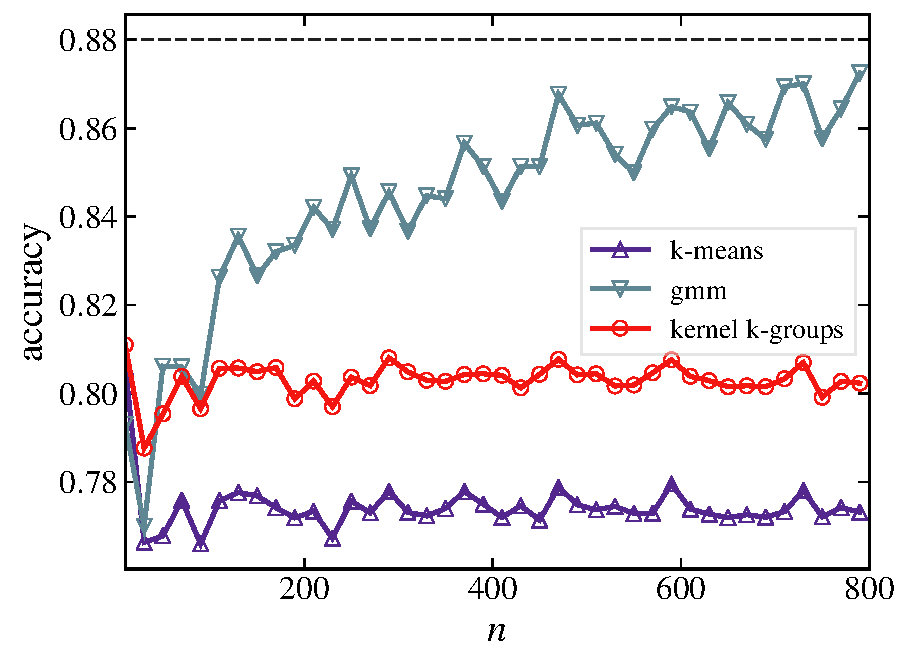
\includegraphics[width=1\textwidth]{gauss_1d.pdf}\\[-2em]
(a)
\end{minipage}
\begin{minipage}{.4\textwidth}
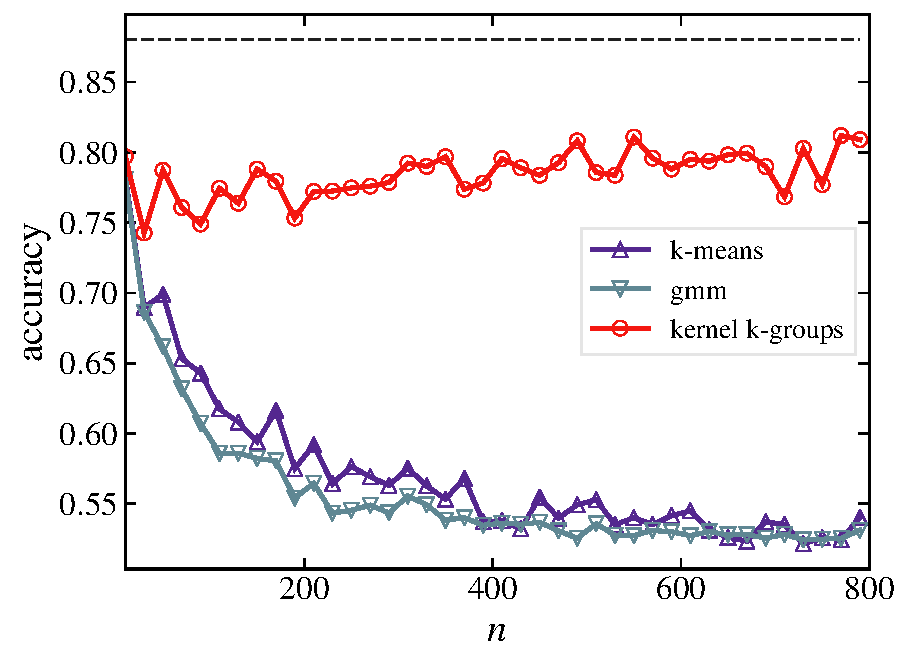
\includegraphics[width=1\textwidth]{loggauss_1d.pdf} \\[-2em]
(b)
\end{minipage}\\[1em]
\begin{minipage}{.37\textwidth}
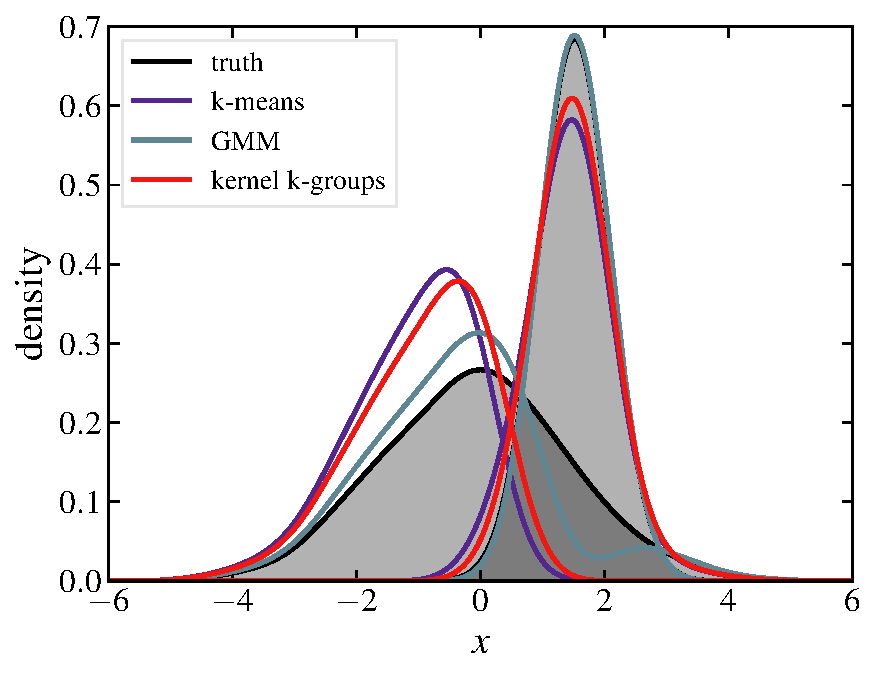
\includegraphics[width=1\textwidth]{normal_density.pdf}\\[-2em]
(c)
\end{minipage}\hspace{2em}
\begin{minipage}{.37\textwidth}
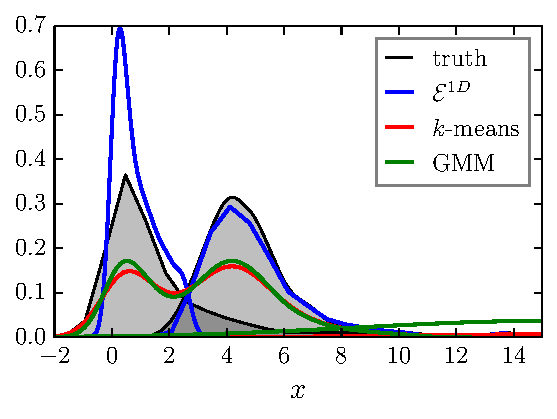
\includegraphics[width=1\textwidth]{lognormal_density.pdf}\\[-2em]
(d)
\end{minipage}
\caption{
\label{fig:1dexperiment}
Clustering one-dimensional data for a two-class problem.
(a) $x \stackrel{iid}{\sim} \tfrac{1}{2} \mathcal{N}(0, 1.5) +
\tfrac{1}{2}\mathcal{N}(1.5,0.3)$. (b) $x \stackrel{iid}{\sim}
\tfrac{1}{2}e^{\mathcal{N}(0, 1.5)} + \tfrac{1}{2} e^{\mathcal{N}(1.5, 0.3)}$.
In both cases we plot the accuracy versus the total number of points.
(c) Kernel density estimation for a single trial with 2000 sampled
points from the
distribution in the case (a). (d) Kernel density estimation in a single
trial with 
2000 points sampled from the distribution in the case (b).
}
\end{figure*}


We first consider one-dimensional data for a two-class problem. We compare
kernel k-groups with k-means and GMM, as illustrated in 
Fig.~\ref{fig:1dexperiment}. The left panels show a mixture of Gaussians, and the right panels show a mixture of log Gaussians (see caption for details).
% have two mixtures of normal and lognormal distributions. 
Notice that in the kernel density estimation plots
for lognormal distribution, only kernel k-groups was able to distinguish
between the two classes. The accuracy results for both density estimation
cases are in Table~\ref{tb:dens}. We remark that kernel k-groups in
this one-dimensional example performed the same as the exact deterministic
Algorithm~\ref{algo1d} introduced in the Appendix.

\begin{table}[h]
\centering
\caption{
\label{tb:dens} Accuracy results for the density
estimation of Fig.~\ref{fig:1dexperiment}d--e.
}
\begin{tabular}{@{}l|ll@{}}
       Method        & normal & lognormal \\ \midrule[.5pt]
        kmeans       & 0.773  & 0.502     \\
         GMM         & \textbf{0.881}  & 0.513     \\
   kernel k-groups   & 0.802  & \textbf{0.847}  
\end{tabular}
\end{table}



Next, we analyze
how the algorithms degrade as the number of dimensions increase.
Consider data from the Gaussian mixture
\begin{equation}
\label{eq:gauss1}
\begin{split}
x  &\stackrel{iid}{\sim} 
\tfrac{1}{2} \mathcal{N}(\mu_1,\Sigma_1) +
\tfrac{1}{2} \mathcal{N}(\mu_2,\Sigma_2), \quad
\Sigma_1=\Sigma_2 = I_D, \\
\mu_1 &= (\underbrace{0,\dotsc,0}_{\times D})^\top, \qquad
\mu_2 = 0.7 (\underbrace{1,\dots,1}_{\times 10},
\underbrace{0,\dots,0}_{\times (D-10)})^\top.
\end{split}
\end{equation}
The Bayes error is fixed as $D$ increases giving an optimal accuracy
of $\approx 0.86$.
We sample $200$ points on each trial. A scatter plot of the last two
dimensions that contains signal in $\mu_2$ is shown in
Fig.~\ref{fig:scatter}a.
The clustering results are shown in Fig.~\ref{fig:plots}a.
We see that 
kernel k-groups and spectral clustering have close
performance, being superior to kernel k-means, k-means, and GMM.
The improvement is noticeable in 
higher dimensions.

\begin{figure*}
\centering
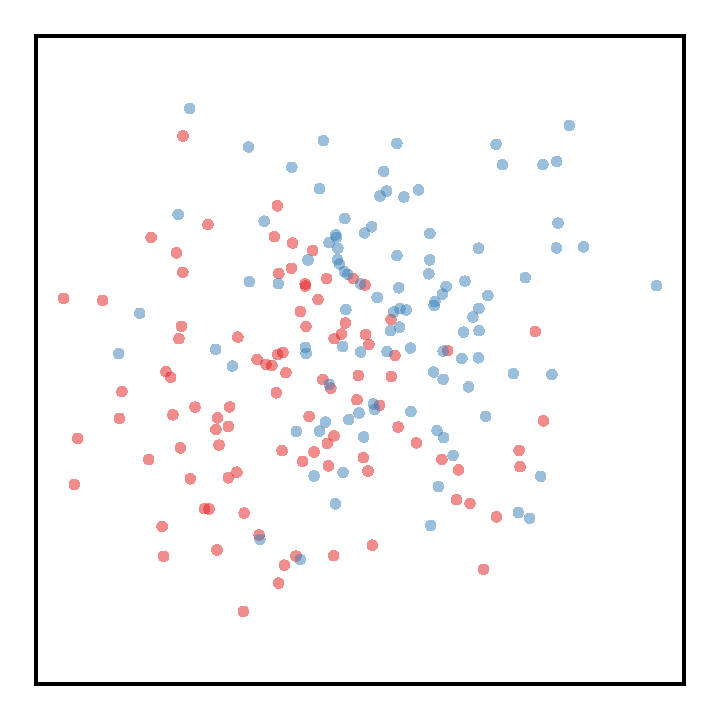
\includegraphics[width=0.19\textwidth]{gauss_means_scatter.pdf}
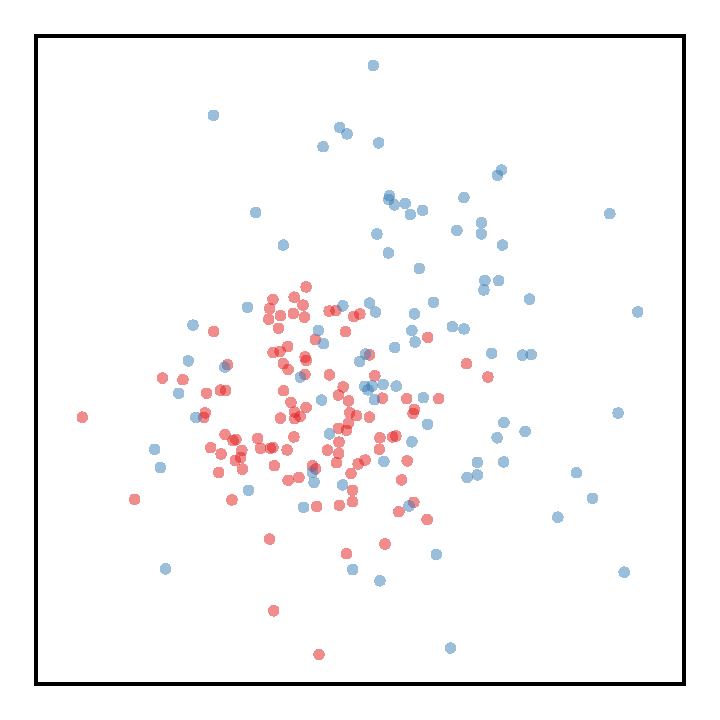
\includegraphics[width=0.19\textwidth]{gauss_cov_scatter.pdf}
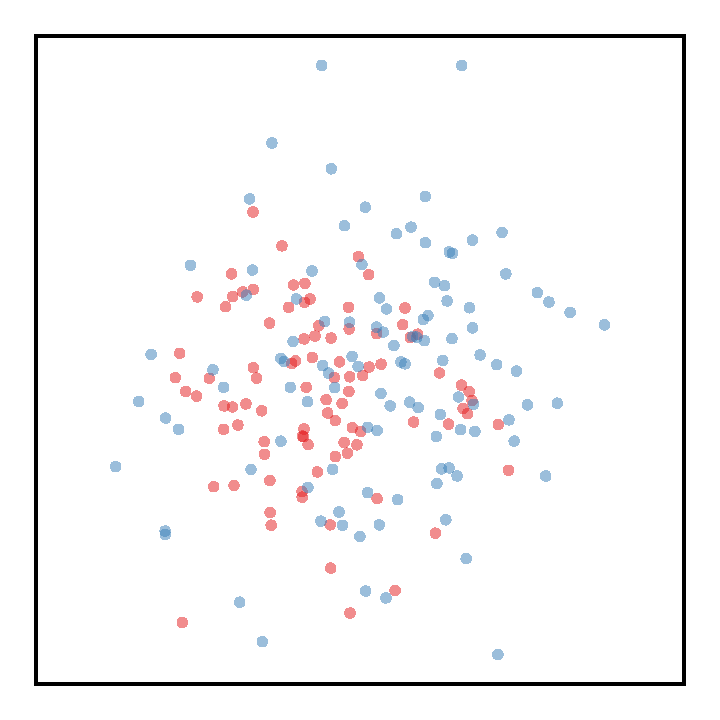
\includegraphics[width=0.19\textwidth]{gauss_diff_metrics.pdf}
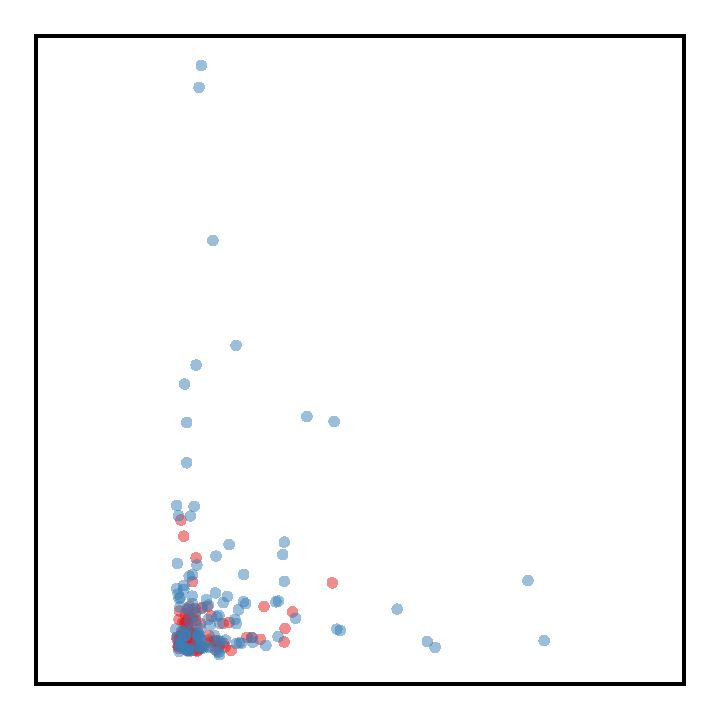
\includegraphics[width=0.19\textwidth]{loggauss_diff_metrics.pdf}
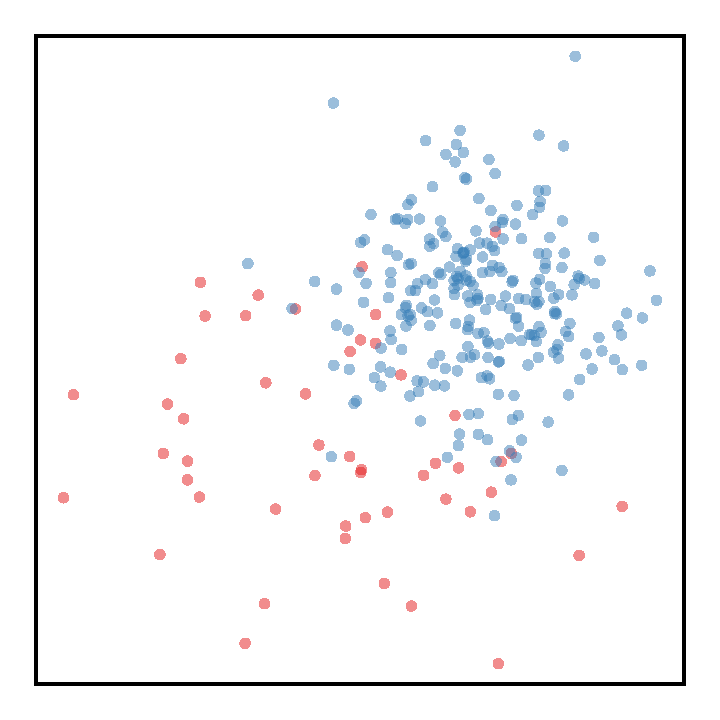
\includegraphics[width=0.19\textwidth]{unbalanced_scatter.pdf}
\put(-500,-8){(a)}
\put(-398,-8){(b)}
\put(-298,-8){(c)}
\put(-195,-8){(d)}
\put(-95,-8){(e)}
\caption{
\label{fig:scatter}
Scatter plot of the last two dimensions where $\mu_2$ has signal.
Each plot has 200 points total.
(a) Data distributed as in \eqref{eq:gauss1}.
(b) Data distributed as in \eqref{eq:gauss2}.
(c) Data distributed as in \eqref{eq:20gauss}.
(d) Parameters as in \eqref{eq:20gauss} but for lognormal mixture.
(e) Data from \eqref{eq:gauss3} with $N = 300$ and $m=200$.
}
\end{figure*}

\begin{figure*}
\centering
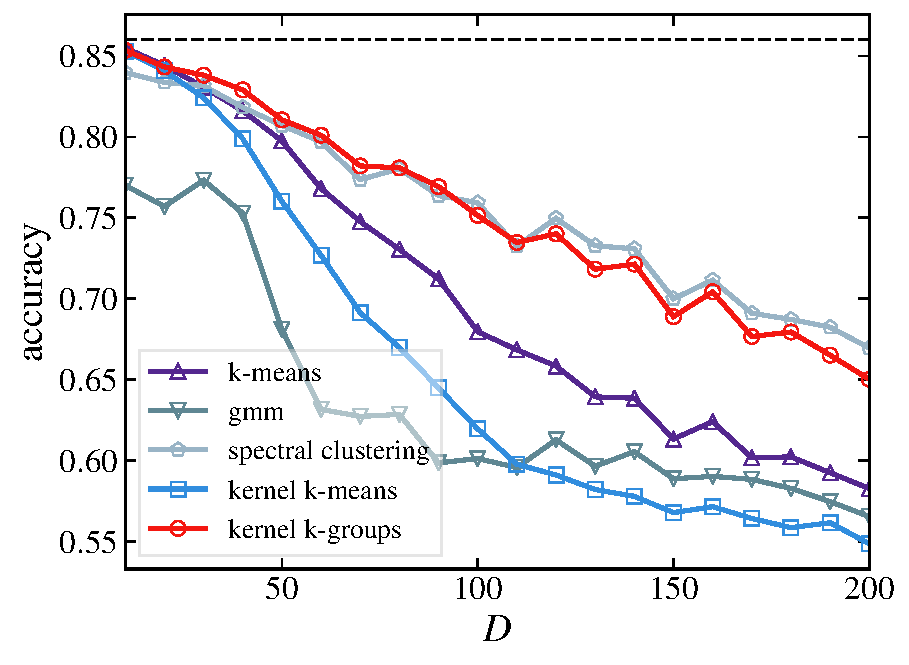
\includegraphics[width=0.33\textwidth]{gauss1.pdf}
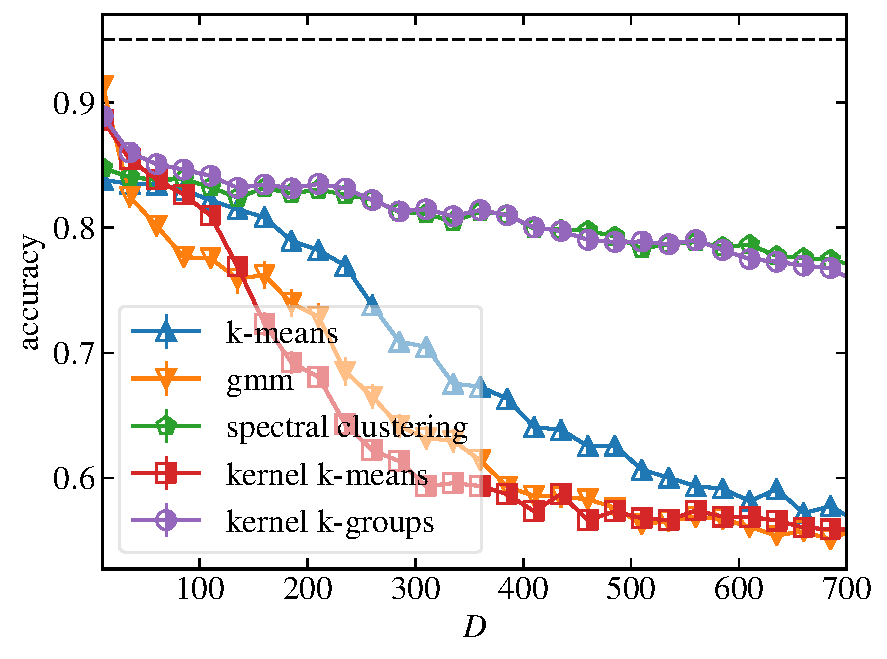
\includegraphics[width=0.33\textwidth]{gauss2.pdf}
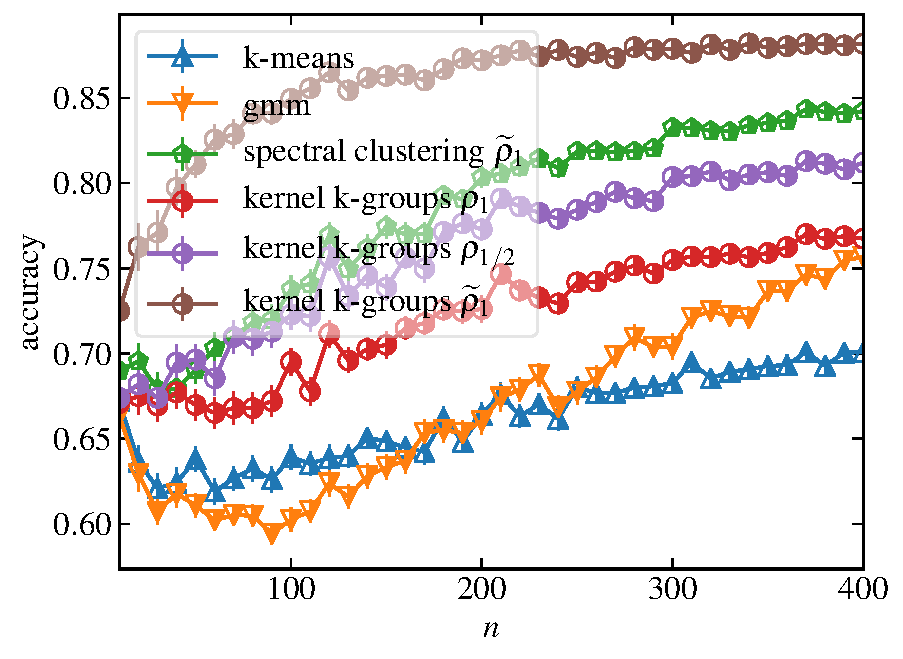
\includegraphics[width=0.33\textwidth]{gauss_n.pdf}
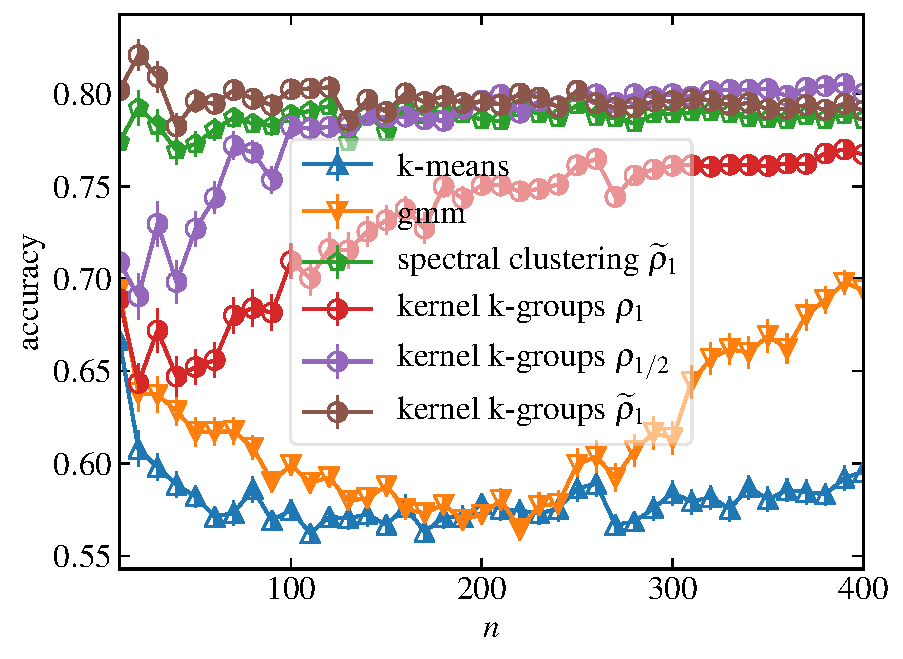
\includegraphics[width=0.33\textwidth]{loggauss_n.pdf}
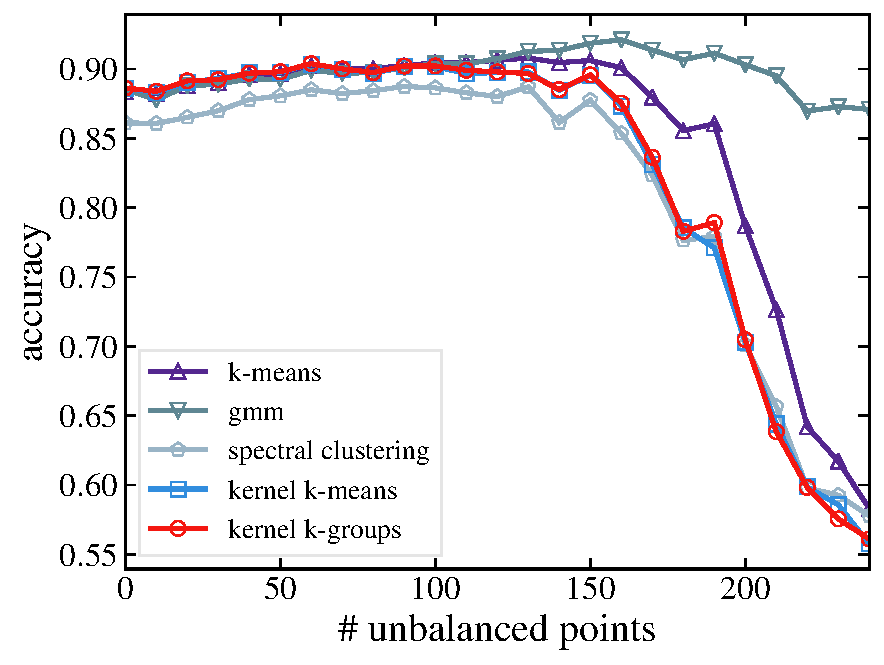
\includegraphics[width=0.315\textwidth]{gauss_unbal.pdf}
\put(-400,130){(a)}
\put(-230,130){(b)}
\put(-50,130){(c)}
\put(-320,-8){(d)}
\put(-140,-8){(e)}
\caption{
\label{fig:plots}
Clustering results associated to the data illustrated in 
Fig.~\ref{fig:scatter}. For each experiment we
perform 100 Monte Carlo runs. Error bars indicate standard error.
(a)
High dimensional Gaussian mixture according to \eqref{eq:gauss1}.
The dashed line is
Bayes accuracy $\approx 0.86$. We use the metric $\rho_1$ in
\eqref{eq:rho_alpha}, which is standard in energy statistics.
(b)
High dimensional Gaussian mixture according to \eqref{eq:gauss2}.
Bayes accuracy $\approx 0.95$. We use $\rho_1$ in \eqref{eq:rho_alpha}.
(c)
Gaussian mixture with parameters \eqref{eq:20gauss}. We increase
the number of sampled points in each trial. We use different
metrics; see \eqref{eq:rho_alpha}--\eqref{eq:rho_hat}. 
Here, kernel k-groups is more accurate than spectral clustering.
(d)
Same experiment as in Fig.~\ref{fig:plots}c but with a 
lognormal mixture with parameters \eqref{eq:20gauss}.
Again, kernel k-groups is more accurate than alternatives.
The plot suggests that neither of these methods are
consistent on this example since Bayes accuracy is $\approx 0.90$.
(e)
Comparison between clustering methods
on unbalanced clusters. The data is normally 
distributed as \eqref{eq:gauss3} where
we vary $m \in [0, 240]$. We use the standard metric $\rho_1$ (see
\eqref{eq:rho_alpha}) from energy statistics.
}
\end{figure*}

Still for a two-class Gaussian mixture as in \eqref{eq:gauss1}, we now choose
different numbers for the  diagonal covariance $\Sigma_2$.
We have $\Sigma_1=I_D$, $\mu_1=(0,\dotsc,0)^\top \in \mathbb{R}^D$,
$\mu_2=(1,\dotsc,1,0,\dotsc,0)^T \in \mathbb{R}^D$, 
with signal in the first $10$ dimensions, and
\begin{equation}
\label{eq:gauss2}
\begin{split}
\Sigma_2 &= \left( \begin{array}{c|c}
\widetilde{\Sigma}_{10} & 0 \\ \hline 
0 & I_{D-10} \end{array}\right), \\
\widetilde{\Sigma}_{10} &= \diag(1.367,  3.175,  3.247,  4.403,  1.249,\\
&\hspace{3.6em}1.969, 4.035,   4.237,  2.813,  3.637).
\end{split}
\end{equation}
We simply chose $10$ numbers uniformly at random on the interval
$[1,5]$ and other choice would give analogous results.
Bayes  accuracy is fixed at $\approx 0.95$. In Fig~\ref{fig:scatter}b
we show a scatter plot of the 9th and 10th dimension.
From Fig.~\ref{fig:plots}b we see that 
all the methods are similarly accurate in low dimensions, but they quickly
degenerate as the number of dimensions increase, except 
kernel k-groups which is much more stable.

Now, consider
$x \stackrel{iid}{\sim} \tfrac{1}{2} \mathcal{N}(\mu_1,\Sigma_1)+
\tfrac{1}{2} \mathcal{N}(\mu_2,\Sigma_2)$
with 
\begin{equation}
\label{eq:20gauss}
\begin{split}
2\Sigma_1 &= \Sigma_2 = I_{20} \\
\mu_1 &= (\underbrace{0,\dotsc,0}_{\times 20})^\top , 
\quad \mu_2 = \tfrac{1}{2} 
(\underbrace{1,\dotsc,1}_{5},\underbrace{0,\dotsc,0}_{15})^\top.
\end{split}
\end{equation}
Bayes accuracy is $\approx 0.90$.  A scatter plot of the 4th and 5th
dimensions is shown in Fig.~\ref{fig:scatter}c.
We increase the sample size $n \in [10, 400]$ and show
the accuracy versus $n$ in Fig.~\ref{fig:plots}c. We compare
kernel k-groups, with different metrics,
to k-means and GMM. We also use
the best metric in this example for spectral clustering.
We notice a superior performance of kernel k-groups 
compared to the other methods.

To consider non-normal data, we sample from the lognormal mixture 
$x \stackrel{iid}{\sim} \tfrac{1}{2} 
e^{\mathcal{N}(\mu_1,\Sigma_1)}+
\tfrac{1}{2} e^{\mathcal{N}(\mu_2,\Sigma_2)}$ with the same
parameters as in \eqref{eq:20gauss}. 
The optimal Bayes accuracy is still $\approx 0.9$.
A scatter plot is in Fig.~\ref{fig:scatter}d and the
results are shown in Fig.~\ref{fig:plots}d.
We use exactly the same metrics as in the normal
mixture of Fig.~\ref{fig:plots}c to illustrate that the 
proposed method still performs accurately.

Finally, we show a limitation of kernel k-groups, which is shared
between 
all the other methods except for GMM.
For highly unbalanced clusters, k-means, spectral
clustering, kernel k-means and kernel k-groups all degenerate
more quickly than GMM. A scatter plot of the first two dimensions
is shown in Fig.~\ref{fig:scatter}e and the clustering results are
in Fig.~\ref{fig:plots}e,
where we generate data according to
\begin{equation}
\label{eq:gauss3}
\begin{split}
x &\stackrel{iid} \sim  
\dfrac{n_1}{2N} \mathcal{N}(\mu_1,\Sigma_1)+
\dfrac{n_1}{2N} \mathcal{N}(\mu_1,\Sigma_1), \\
\mu_1 &= (0,0,0,0)^\top , \quad
\mu_2 = 1.5\times (1,1,0,0)^\top, \\
\Sigma_1 &= I_4, \quad
\Sigma_2 = \left( 
\begin{array}{c|c} 
\tfrac{1}{2} I_2 & 0  \\ \hline
0 & I_2 
\end{array}\right), \\
n_1 &= N - m, \quad  n_2 = N + m, \quad N=300.
\end{split}
\end{equation}
We then increase $m \in [0,240]$ making
the clusters progressively more unbalanced.
For highly unbalanced clusters, we see that GMM performs better than
the other methods, which have basically similar performance.
Based on this experiment, an interesting problem would be to
extend kernel k-groups to account for unbalanced clusters.

In Fig.~\ref{fig:2dscatter} we show examples of two-dimensional
datasets whose clustering results are shown in Table~\ref{tb:cigar_circle}.
For kernel k-means and kernel k-groups we initialize at random.
We see that both methods perform closely, with higher accuracy
than the other ones.

\begin{figure}
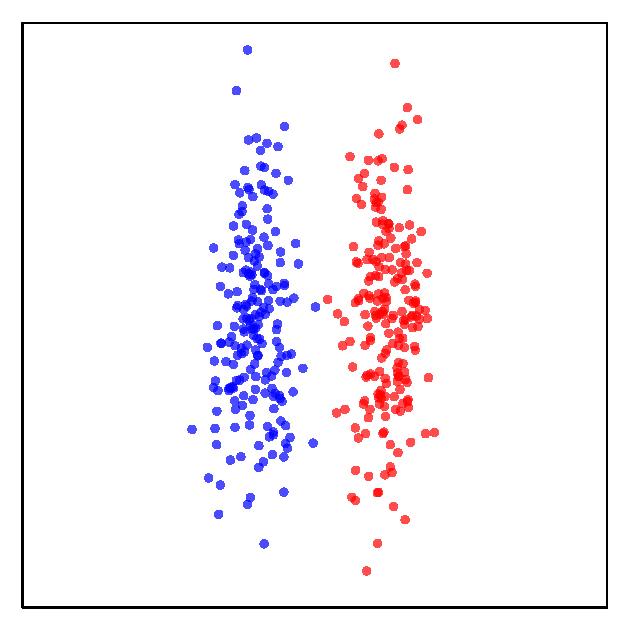
\includegraphics[width=.24\textwidth]{2cigars.pdf}
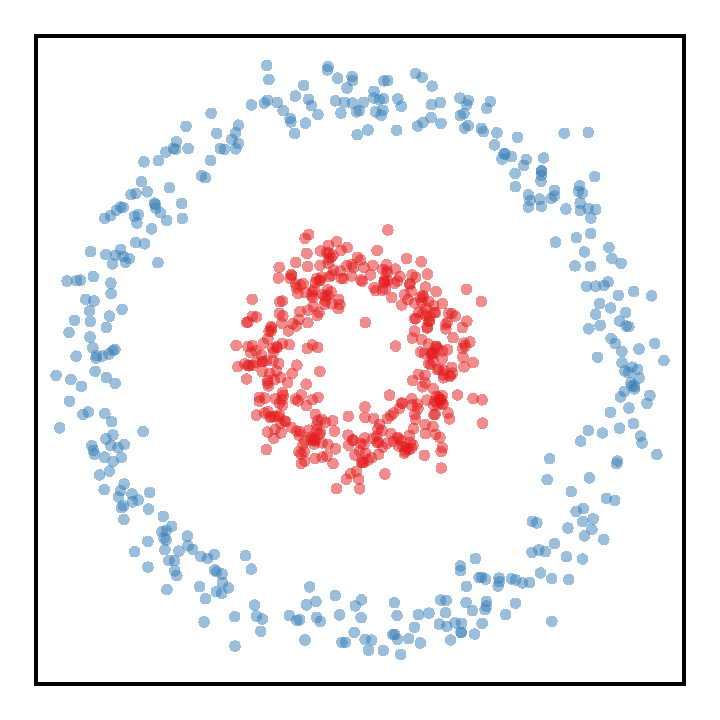
\includegraphics[width=.24\textwidth]{2circles.pdf}
\put(-240,-8){(a)}
\put(-110,-8){(b)}
\caption{
\label{fig:2dscatter}
(a) Data distributed as 
$x \stackrel{iid}{\sim}
\tfrac{1}{2}\mathcal{N}(\mu_1,\Sigma_1)+
\tfrac{1}{2}\mathcal{N}(\mu_1,\Sigma_1)$, 
$\mu_1= (0,0)^\top$, 
$\mu_2 = (6.5, 0)^\top$ and 
$\Sigma_1 = \Sigma_2 = \diag(1, 20)$. We sample $800$ points.
(b) Concentric circles with radius $r_1 = 1$ and $r_2 = 3$, with 
noise $0.2 \cdot \mathcal{N}(0, I_2)$. We sample 
800 points with probability $1/2$ for each class.
} 
\end{figure}

\begin{table}
\caption{
\label{tb:cigar_circle}
Clustering the data from Fig.~\ref{fig:2dscatter}.
For spcetral clustering, kernel k-means and kernel k-groups we use
the metric $\widetilde{\rho}_2$ (see \eqref{eq:rho_tilde}) for the data
in Fig.~\ref{fig:2dscatter}a, while $\widehat{\rho}_1$ (see \eqref{eq:rho_hat})
for the data in Fig.~\ref{fig:2dscatter}b. We have 800
points on each trial and 30 Monte Carlo runs for both datasets.
}
\centering
\begin{tabular}{@{}l|ll|ll@{}}
                   & \multicolumn{2}{c|}{Fig.~\ref{fig:2dscatter}a}  &
                     \multicolumn{2}{c}{Fig.~\ref{fig:2dscatter}b}  \\
       Method      & Accuracy & SEM     & Accuracy & SEM \\ \midrule[.5pt]
        kmeans       & 0.533 & 0.005  & 0.521   & 0.003 \\
         GMM         & 0.929 & 0.029  & 0.533   & 0.004 \\
 spectral clustering & 0.577 & 0.010  & 0.725   & 0.003 \\
    kernel k-means   & \textbf{1.000} & 0.000  & \textbf{1.000}   & 0.000 \\
   kernel k-groups   & \textbf{1.000} & 0.000  & \textbf{1.000}  & 0.000  
\end{tabular}
\end{table}


%%%%%%%%%%%%%%%%%%%%%%%%%%%%%%%%%%%%%%%%%%%%%%%%%%%%%%%%%%%%%%%%%%%%%%%%%%%%%%%
\subsection{Real Data Experiment}

We consider the dermatology dataset \cite{Dua2017,Guvenir1998}
which has 366 data points, each with 34 attributes where 33 are
linear valued and one is categorical. There are 8 data points with
missing entries in the ``age'' column. We complete the missing entries
with the mean of the entire column, and then we normalize the entire
dataset to zero mean and unit variance. There are  a total of $6$ classes,
and this is a challenging clustering problem. We refer the reader
to \cite{Dua2017,Guvenir1998} for a complete description of the dataset, 
and also to \cite{RizzoClustering} where this dataset was previously
analyzed. In Table~\ref{tb:dermatology} we show the results of kernel
k-groups using the metric \eqref{eq:rho_alpha} with $\alpha=1/2$.
We show the number of points assigned to each class while indicating
the actual class that points belong to. In Table~\ref{tb:dermatology_accuracy}
we show this experiment using several clustering methods, and we also
compare with the results from \cite{RizzoClustering} and \cite{Kgroups}
on this same data. Our results provide an improvement in comparison
to all the other methods and also the analysis
of \cite{RizzoClustering}.

\begin{table}
\caption{
\label{tb:dermatology}
Clustering the dermatology 
dataset of \cite{Dua2017,Guvenir1998} with kernel k-groups
using the metric $\rho_{1/2}$ (see \eqref{eq:rho_alpha}) from energy
statistics. The table below should be compared with Table~2 of
\cite{RizzoClustering}, for which our results are slightly more accurate.
See also Table~\ref{tb:dermatology_accuracy} below for clustering metrics.
The classes in the vertical indicates the ground truth and the classes
in the horizontal correspond to the classification
obtained by kernel k-groups. We show the estimated number of points
for each class.
}
\centering
\begin{tabular}{@{}l|llllll|l@{}}
%\toprule[1pt]
class & 1 & 2 & 3 & 4 & 5 & 6 & $\#$ cases \\ \midrule[.5pt]
   1   & 112 & 0  & 0  & 0  & 0  & 0  &  112  \\
   2   &  0  & 50 & 0  & 11 & 0  & 0  &   61  \\
   3   &  0  & 0  & 72 & 0  & 0  & 0  &   72  \\
   4   &  0  & 2  & 0  & 47 & 0  & 0  &   49  \\
   5   &  0  & 0  & 0  & 1  & 51 & 0  &   52  \\
   6   &  0  & 0  & 0  & 0  & 0  & 20 &   20  \\ \midrule[.5pt]
total & 112 & 52 & 72 & 59 & 51 & 20 &  366 %\\ \bottomrule[1pt] 
\end{tabular}
\end{table}

\begin{table}
\caption{
\label{tb:dermatology_accuracy}
For the dataset \cite{Dua2017,Guvenir1998} (see also
Table~\ref{tb:dermatology}) we show the accuracy \eqref{eq:accuracy} and
the adjusted Rand index (aRand) of several methods.
In \cite{RizzoClustering} the authors 
obtained $\textnormal{aRand}=0.9195$ using an energy statistics
based method, while \cite{Kgroups} obtains $\textnormal{aRand}=0.9188$ 
where points with missing
entries are removed. Below we complete the missing entries with the mean.
If we remove the points with missing entries, kernel k-groups provides an
improvement of $\textnormal{accuracy}=0.9637$ and $\textnormal{aRand}=0.9396$.
}
\centering
\begin{tabular}{@{}l|ll@{}}
       Method      & Accuracy & aRand \\ \midrule[.5pt]
        kmeans       & 0.713 & 0.690 \\
         GMM         & 0.877 & 0.840 \\
 spectral clustering & 0.954 & 0.912 \\
    kernel k-means   & 0.751 & 0.851 \\
   kernel k-groups   & \textbf{0.962} & \textbf{0.936}
\end{tabular}
\end{table}


%%%%%%%%%%%%%%%%%%%%%%%%%%%%%%%%%%%%%%%%%%%%%%%%%%%%%%%%%%%%%%%%%%%%%%%%%%%%%%%
\section{Conclusion}
\label{sec:conclusion}

We proposed a formulation to clustering based on a weighted
version of energy statistics, 
valid for arbitrary spaces of negative type.
Our mathematical formulation of energy clustering 
reduces to a QCQP in the associated RKHS, as demonstrated in 
Proposition~\ref{th:qcqp3}.
We showed that the optimization problem
is equivalent
to kernel k-means, once the kernel is fixed, and also
to several graph partitioning problems.
%Energy statistics, however, fixes
%a family of standard kernels in Euclidean space, and
%more general kernels 
%on spaces of negative type can also be obtained.

We extended Hartigan's method to kernel spaces and proposed
Algorithm~\ref{algo}, which we called kernel k-groups.
This method was compared to kernel k-means and spectral clustering, besides
k-means and GMM. Our numerical results show a superior performance of the
proposed method, specially in high dimensions.
We stress that kernel k-groups has the same complexity of kernel k-means.

Kernel k-groups suffers a limitation shared by kernel k-means and spectral
clustering which involves highly unbalanced
clusters. An interesting problem  that we leave open 
is to extend the method to such 
situations.
Finally, kernel methods can benefit from sparsity and
fixed-rank approximations of the Gram matrix, and there is plenty
of room to make kernel k-groups more scalable.


% @gui: better, but still important to have another paragraph between those connecting it to the existing literature.  compare this work with 3-4 other works explicitly stating the difference.








% if have a single appendix:
%\appendix[Proof of the Zonklar Equations]
% or
\appendix  % for no appendix heading
% do not use \section anymore after \appendix, only \section*
% is possibly needed

% use appendices with more than one appendix
% then use \section to start each appendix
% you must declare a \section before using any
% \subsection or using \label (\appendices by itself
% starts a section numbered zero.)
%


%\appendices
%\section{Proof of the First Zonklar Equation}
%Appendix one text goes here.

% you can choose not to have a title for an appendix
% if you want by leaving the argument blank
%\section{}
%Appendix two text goes here.

\section*{Two-Class Problem in One Dimension}
\label{sec:twoclass}

Here we consider the simplest possible case which
is one-dimensional data and a two-class problem. We propose
an algorithm that does not depend on initialization. We used this simple
scheme to compare with kernel k-groups given
in algorithm \ref{algo}. Both algorithms have the same clustering
performance in the one-dimensional examples that we tested.

Let us fix 
$\rho(x,y) = |x - y|$ according to the standard energy distance. We also
fix the weights $w(x) = 1$ for every data point $x$. We can
thus 
compute the function
\eqref{eq:g_def} in $\OO(n \log n)$ and minimize
$W$ directly.
This is done by noting that
\begin{equation}
\begin{aligned}
|x - y|  &= (x-y)\Ind{x \ge y} -
(x-y) \Ind{x < y}  \\
&= 
x \left( \Ind{x \ge y} - \Ind{x < y} \right)  + 
y \left( \Ind{y > x} - \Ind{y \le x} \right)  
\end{aligned}
\end{equation}
where we have the indicator function defined by
$\Ind{A}=1$ if $A$ is true, and $\Ind{A}=0$ otherwise.
Let $\C$ be a partition with
$n$ elements. Using the above distance we have
\begin{equation}
\label{eq:g_ind}
 g\left(\C,\C\right) =  \dfrac{1}{n^2}  
\sum_{x \in \C} 
\sum_{y \in \C} 
x \left(
\Ind{x \ge y} + \Ind{y > x} - 
\Ind{x \ge y}-\Ind{x < y} \right) .
\end{equation}
The sum over $y$ can be eliminated since each term in
the parenthesis is simply counting the number of elements in $\C$ that satisfy
the condition of the indicator function. Assuming
that we first order the data in $\C$, obtaining
$\tC = [ x_j \in \C: x_1 \le x_2 \le \dotsm \le x_{n}]$, we
get
\begin{equation}
\label{eq:g1d}
g\big(\tC, \tC \big) = 
\dfrac{2}{n^2} \sum_{\ell=1}^n (2\ell - 1 - n) x_\ell .
\end{equation}
Note that the cost of computing
$g\big( \tC, \tC \big)$
is $\OO(n)$ and the cost of
sorting the data
is at the most $\OO(n\log n)$.
Assuming that each partition is ordered,
$\mathbb{X} = \bigcup_{j=1}^k \tC_j$,
the within energy dispersion
can be written explicitly as
\begin{equation}
\label{eq:w1d}
W\big( \tC_1,\dotsc,\tC_k \big) = 
\sum_{j=1}^k \sum_{\ell=1}^{n_j} \dfrac{2\ell - 1 - n_j}{n_j} \, x_\ell.
\end{equation}

For a two-class problem we can use the formula
\eqref{eq:w1d} to cluster the data
through a simple algorithm
as follows. We first order
the entire dataset, $\mathbb{X} \to \widetilde{\mathbb{X}}$. Then
we compute \eqref{eq:w1d} for each possible split of $\widetilde{\mathbb{X}}$
and pick the point which gives the minimum value of $W$.
This procedure is described in Algorithm~\ref{algo1d}.
Note that this algorithm is deterministic,
however,
it only works for one-dimensional data with Euclidean distance. Its total
complexity is $\OO(n\log n + n^2) = \OO(n^2)$.


\begin{algorithm}[h]
\vspace{.5em}
\begin{algorithmic}[1]
\INPUT data $\mathbb{X}$
\OUTPUT label matrix $Z$
\STATE sort $\mathbb{X}$ obtaining
$\widetilde{\mathbb{X}}= [ x_1,\dotsc,x_n ]$
    \FOR{$j\in [ 1,\dotsc,n ]$}
        \STATE $\tC_{1,j} \leftarrow [x_i: i=1,\dotsc,j]$
        \STATE $\tC_{2,j} \leftarrow [x_i : i=j+1,\dotsc,n]$
        \STATE
            $W^{(j)} \leftarrow W \big( \tC_{1,j},\tC_{2,j}\big)$
            \hfill (see \eqref{eq:w1d})
    \ENDFOR
    \STATE $j^\star \leftarrow \argmin_j W^{(j)}$
	\FOR{$j \in [1,\dotsc,n]$}
		\IF{ $j\le j^\star$ }
    		\STATE $Z_{j\bullet} \leftarrow (1,0) $
        \ELSE
			\STATE $Z_{j\bullet} \leftarrow (0,1)$
		\ENDIF
	\ENDFOR
\end{algorithmic}
\caption{
\label{algo1d}
Clustering algorithm to
find local solutions to the optimization
problem \eqref{eq:minimize}
for a two-class problem in one dimension. 
}
\end{algorithm}



% use section* for acknowledgment
\ifCLASSOPTIONcompsoc
  % The Computer Society usually uses the plural form
  \section*{Acknowledgments}
\else
  % regular IEEE prefers the singular form
  \section*{Acknowledgment}
\fi

We would like to thank Carey Priebe for discussions.
We would like to acknowledge the support of the Transformative
Research Award (NIH \#R01NS092474) and  the Defense Advanced Research Projects
Agency’s (DARPA) SIMPLEX program through SPAWAR contract N66001-15-C-4041.



% Can use something like this to put references on a page
% by themselves when using endfloat and the captionsoff option.
\ifCLASSOPTIONcaptionsoff
  \newpage
\fi



% trigger a \newpage just before the given reference
% number - used to balance the columns on the last page
% adjust value as needed - may need to be readjusted if
% the document is modified later
%\IEEEtriggeratref{8}
% The "triggered" command can be changed if desired:
%\IEEEtriggercmd{\enlargethispage{-5in}}

% references section

% can use a bibliography generated by BibTeX as a .bbl file
% BibTeX documentation can be easily obtained at:
% http://mirror.ctan.org/biblio/bibtex/contrib/doc/
% The IEEEtran BibTeX style support page is at:
% http://www.michaelshell.org/tex/ieeetran/bibtex/
%\bibliographystyle{IEEEtran}
% argument is your BibTeX string definitions and bibliography database(s)
%\bibliography{IEEEabrv,../bib/paper}
%
% <OR> manually copy in the resultant .bbl file
% set second argument of \begin to the number of references
% (used to reserve space for the reference number labels box)


\bibliographystyle{unsrt}
%\bibliographystyle{abbrvnat}
\bibliography{biblio.bib}


% biography section
% 
% If you have an EPS/PDF photo (graphicx package needed) extra braces are
% needed around the contents of the optional argument to biography to prevent
% the LaTeX parser from getting confused when it sees the complicated
% \includegraphics command within an optional argument. (You could create
% your own custom macro containing the \includegraphics command to make things
% simpler here.)
%\begin{IEEEbiography}[{\includegraphics[width=1in,height=1.25in,clip,keepaspectratio]{mshell}}]{Michael Shell}
% or if you just want to reserve a space for a photo:

\begin{IEEEbiography}{Guilherme Fran\c ca}
Biography text here.
\end{IEEEbiography}

% if you will not have a photo at all:
\begin{IEEEbiographynophoto}{Maria Rizzo}
Biography text here.
\end{IEEEbiographynophoto}

% insert where needed to balance the two columns on the last page with
% biographies
%\newpage

\begin{IEEEbiographynophoto}{Joshua T.~Vogelstein}
I received a B.S degree from the Department of Biomedical Engineering (BME) at Washington University in St. Louis, MO in 2002, a M.S. degree from the Department of Applied Mathematics and Statistics (AMS) at Johns Hopkins University (JHU) in Baltimore, MD in 2009, and a Ph.D. degree from the Department of Neuroscience at JHU in 2009. I was a Postdoctoral Fellow in AMS@JHU from 2009 until 2011, at which time I was appointed an Assistant Research Scientist, and became a member of the Institute for Data Intensive Science and Engineering. I spent 2 years at Information Initiative at Duke University, before coming home to my current appointment as Assistant Professor in BME@JHU, and core faculty in both the Institute for Computational Medicine and the Center for Imaging Science, as well as a member of the Kavli Neuroscience Discovery Institute. I married my kindergarten sweetheart in the summer of 2014. 

My primary research interest is to extend and fuse statistical machine learning and big data science to address the most important brain science and mental health questions of our time, particularly  connectomics. Our group’s research has been featured in a number of prominent scientific and engineering journals and conferences including Nature, Nature Methods, Science, Cell, PNAS, Science Translational Medicine, JMLR, PAMI, Annals of Applied Statistics,  NIPS, and SIAM Journal of Matrix Analysis and Applications. In 2011, I co-founded the Open Connectome Project which expanded in 2015 to be NeuroData, whose mission is to enable terascale neuroscience for everyone. All our work is conducted according to the highest standards of open science.
\end{IEEEbiographynophoto}

% You can push biographies down or up by placing
% a \vfill before or after them. The appropriate
% use of \vfill depends on what kind of text is
% on the last page and whether or not the columns
% are being equalized.

%\vfill

% Can be used to pull up biographies so that the bottom of the last one
% is flush with the other column.
%\enlargethispage{-5in}



% that's all folks
\end{document}


